% tADRguide.tex
% v1.0 released January 2013

\documentclass{tADR2e}

% The following packages can be found on http:\\www.ctan.org
\usepackage{caption}
\usepackage{color}
\usepackage{graphicx} % for pdf, bitmapped graphics files
%\usepackage{epsfig} % for postscript graphics files
\usepackage{mathptmx} % assumes new font selection scheme installed
\usepackage{amsmath} % assumes amsmath package installed
\usepackage{amssymb}  % assumes amsmath package installed
\usepackage{mathrsfs}
\DeclareMathOperator*{\argmin}{argmin}
\usepackage{algorithm}
\usepackage{algpseudocode}  %\usepackage[noend]{algpseudocode}
\algtext*{EndWhile}% Remove "end while" text
\algtext*{EndIf}% Remove "end if" text
\usepackage{booktabs}
\usepackage{multirow}
\usepackage{proof}
\newtheorem{property}{Property}
\usepackage[numbers]{natbib}
\algnewcommand\algorithmicinput{\textbf{Input:}}
\algnewcommand\INPUT{\item[\algorithmicinput]}
\algnewcommand\algorithmicoutput{\textbf{Output:}}
\algnewcommand\OUTPUT{\item[\algorithmicoutput]}
\makeatletter
\makeatother
\usepackage{hyperref}
\usepackage{xcolor}
\hypersetup{
    colorlinks,
    linkcolor={red!80!black},
    citecolor={blue!80!black},
    urlcolor={blue!80!black}
}


% Math shortcuts :
\newcommand\real{\mathbb{R}}
\newcommand\p{\mathbf{p}}
\newcommand\pii{\mathbf{p_{i,i+1}}}
\newcommand\pij{\mathbf{p_{i,j}}}
\newcommand\gT{\tilde{g}^T}
\newcommand\g{\tilde{g}}
\newcommand\CS{\mathcal{C}}
\newcommand\dimCS{n_\mathbf{C}}
\newcommand\body{{\cal B}}
\newcommand\Sone{\mathbf{S}^1}
\newcommand\Sthree{\mathbf{S}^3}
\newcommand\conf{\mathbf{q}}
\newcommand\xx{\mathbf{x}} % \x already defined in the class
\newcommand\cost{C}
\newcommand\weight{W}
\newcommand\translation{\mathbf{t}}
\newcommand\tcolli{t_{coll\ i}}
\newcommand\po{\mathbf{po}}
\newcommand\Jf{{J_f}}
\newcommand\kernel{\mbox{Ker }}

%%%%%%%%%%%%%%%%%%%%%%%%%%%%%%%%%%%%%%%%%%%%%%%%%%%%%%%%%%%%%%%%%%%%%%%%%%%%%%%%
\begin{document}
\graphicspath{{images/}}



\title{A simple path optimization method for motion planning$^{1}$ \thanks{$^{1}$Note for the reviewers: 
This paper is an extended version of a paper submitted to IEEE ICRA 2016~\cite{pathOptimICRA_HAL}. The 
current version includes a problem formulation, a convergence analysis and many experimental results (including an 
industrial example) which are absent from the conference version.}}	

\author{Myl\`{e}ne Campana$^{\ast}$ \thanks{$^\ast$Corresponding author. Email: \href{mailto:mcampana@laas.fr}{mcampana@laas.fr}}, Florent Lamiraux and Jean-Paul Laumond
\\\vspace{6pt}
{\em{LAAS-CNRS, 7 av. Colonel Roche, 31400 Toulouse, FRANCE}}
}
\maketitle



\begin{abstract}
Most algorithms in probabilistic sampling-based path planning compute 
collision-free paths made of straight line segments lying in the configuration 
space. Due
to the randomness of sampling, the paths make detours that need to be optimized.
The contribution of this paper is to propose a basic gradient-based (GB) algorithm 
that transforms a polygonal collision-free path into a shorter one.
While requiring only collision 
checking, and not any time-consuming obstacle distance computation nor geometry 
simplification, we constrain only part of the configuration variables 
that may cause a collision, and not entire configurations. As a result, parasite motions that are not useful for the problem resolution are reduced without any 
assumption.
Experimental results include navigation and manipulation tasks, 
e.g. a manipulator arm filling boxes and a PR2 robot working in a kitchen 
environment. Comparisons with a random shortcut optimizer and a partial 
shortcut have also been studied.

% few parameter tuning REMOVED

\medskip

\begin{keywords}path optimization; motion planning; robotics
\end{keywords}\medskip

\end{abstract}


\section{Introduction}
Motion planning for systems in cluttered environments has been addressed for more
than thirty years~\cite{ref-motionplan}. 
To explore the connected components of collision-free configuration spaces, pioneering 
contributions in the 90’s introduced certain levels of random searches, i.e. random walks in~\cite{potentielBarraquandLatombe}, random sampling in 
~\cite{KavrakiLatombePRM} and~\cite{LaValleKuffnerRRT}. Today most motion planners are inspired by these seminal approaches.
The main issue using these techniques is that the computed path makes unnecessary 
detours and needs to be post-processed before being executed by a virtual or real 
robot. Alternative strategies exist however.
\begin{itemize}
\item Planning by path-optimization~\cite{itomp2012},~\cite{voronoiOMP} where
obstacle avoidance is handled by constraints or cost using computation of the
nearest obstacle distance. Most of these planners are using non-linear
optimization~\cite{BettsNonlinopt} under constraints. Such planners provide close-to-optimality paths and have smaller time computation
for easy problems, but they are mostly unable to solve narrow passage issues.
 
\item Optimal random sampling~\cite{KaramanPRMstarRRTstar} are also close to an
optimal solution, but computation time is significantly higher than classical
approaches.
\end{itemize}

In this paper, we propose a method aimed at shortening path length after a path
planning step. Note that we do not address path planning, but that we take the
result of a probabilistic motion planner as the input to our path optimization 
method.

For this shortening purpose, random shortcut (RS) methods are
still very 
popular~\cite{Sekhavat-Svestka1998,Geraerts04clearancebased,HauserFastSmooth}. 
However, RS requires fine 
tuning of the termination condition and is no efficient for long 
trajectories where only a minor part needs to be optimized, 
as in (Figure~\ref{local_box_optim}).
(Figure~\ref{decoupled_DOF_optimization}) presents another situation where RS 
will always fail to optimize the initial path, since it cannot decouple the 
robot degrees of freedom (DOF) on which the optimization occurs. This problem is 
addressed by our method.

\begin{figure}
	\centering
	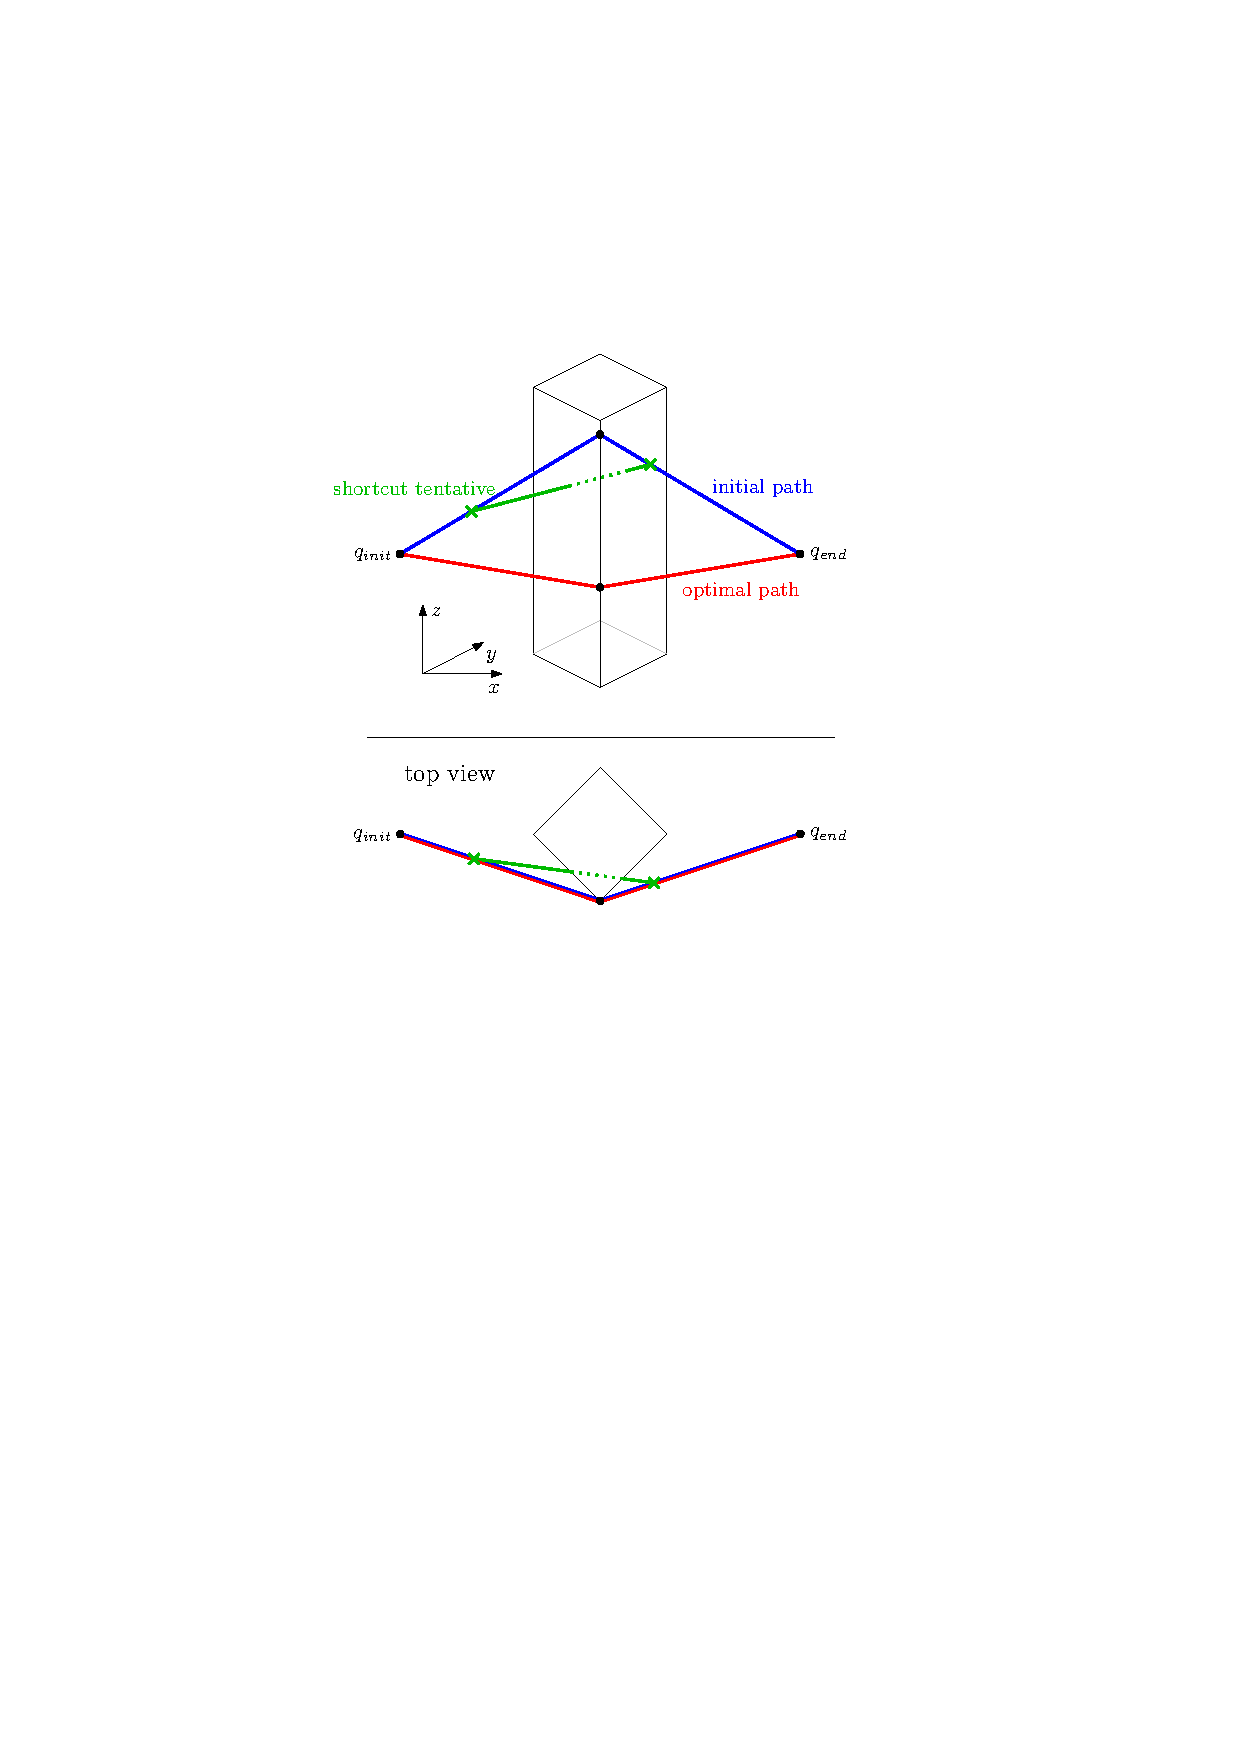
\includegraphics[width=7.5cm]{decoupled_DOF_optimization.pdf}
	\caption{Example of a path in $\real^3$ which random shortcut will never manage to 
	optimize: each shortcut tentative will provide a collision or will not 
	decrease the path length. The optimal path belongs to the $x-y$ plane 
	containing $\conf_{init}$ and $\conf_{final}$.}
	\label{decoupled_DOF_optimization}
\end{figure}

On the other hand, numerical
optimization methods like CHOMP~\cite{chompIjrr} can be used as a
post-processing step. They have clear termination conditions, but collision
avoidance is handled by inequality constraints sampled at many points along
the trajectory. These methods therefore require a pre-processing step of the
robot (and/or environment) model in order to make 
it simpler:~\cite{chompIjrr} covers PR2 bodies with spheres, 
while~\cite{convexOptimMotplan} needs to decompose objects into convex subsets.

Finally it should be noticed that optimality in robot motion is a notion that should be clarified. Most of the time motion planners provide an optimized motion, which is not optimal at all, but is the output of a given optimization method. When optimal motions exist, numerical
algorithms mostly fail in accounting for their combinatorial structure. In addition, optimization algorithms bypass (not overcome) the question of the existence of optimal motions~\cite{LaumondOptim}. In that perspective, a path optimization algorithm has to be evaluated with respect to other existing optimization techniques, from qualitative properties and from computational performance.

The idea of our method is to find a good trade-off between
the simplicity of “blind” methods like shortcut algorithm,
and the complexity of distance based optimization techniques.
The method iteratively shortens the initial path with gradient-based information.
When a collision is detected at a given iteration, the method backtracks to the
latest valid iteration and inserts a one-dimensional constraint
between the objects detected in collision. Only collisions between objects are 
evaluated, therefore no pre-processing of the
robot or environment models is necessary to increase distance computation speed. 
Respecting the problem geometry also 
preserves that a solution can still be found, e.g. for narrow passages as holes or 
grippers. The method is also repeatable since no randomness is introduced. The underlying optimization algorithm is a quadratic program.

Related work is presented in Section II. Section III explains how the 
path-optimizer works, from the formulation of the problem to the implemented
algorithm. Finally, we conclude on experimental results in Section IV.

\section{RELATED WORK}
Previous work on path optimization has been conducted. CHOMP algorithm~\cite{chompIjrr} optimizes an initial guess provided as
input. It minimizes a time invariant cost function using efficient covariant
Hamiltonian gradient descent. The cost is quantified by non-smooth parts (with
high velocities) and an obstacle avoidance term, provided by the distance to the 
nearest obstacle for each iteration of the trajectory. Calculating these nearest 
distances however is time-consuming because the distances between all pairs of 
objects must be computed at each time step along the path. To reduce the 
computation time, the method starts by building offline a map of distances that 
will be called during the optimization at the requested time. Besides, meshes 
are pre-processed into bounding spheres so that distances are computed faster 
at the cost of a geometry approximation.

STOMP method~\cite{KalakrishnanStomp} avoids to compute an 
explicit gradient for cost optimization using a stochastic analysis of local 
random samples. But as for CHOMP, the obstacle cost term requires a voxel map to 
perform its Euclidean Distance Transforms, and represents the robot bodies with 
overlapping spheres. Such technique provides lots of distance and penetration 
information but remains very time consuming and is not as precise as some 
distance computation techniques based on the problem meshes as 
Gilbert-Johnson-Keerthi~\cite{gilbertGjk}.

Some optimization-based planners may not require an initial guess but some naive 
straight-line manually or randomly-sampled initialization as 
TrajOp~\cite{SchulmanConvexOptim}. Its trajectory is iteratively optimized with 
sequential convex optimization by minimizing at each step its square length, 
linear and non-linear constraints considered as penalties. To compute the 
collision-constraints, nearest obstacle distances are calculated at each discrete 
time of the trajectory vector. This can be a burden for a high-dimensional robot 
or a complex environment as we propose to use, and may be compensated with a 
short path composed of only one or two waypoints.


The elastic strips framework~\cite{BrockElasticStrips} is also an optimization 
based method. The path is modeled as a spring and obstacles give rise to a 
repulsive potential field. Although designed for on-line control purposes, this 
method may be used for path shortening. In this case however, the number of 
distance computation is very high. The authors also proposed to approximate the 
robot geometry by spheres.

Some heuristics use random shortcuts on the initial guess combined with a 
trajectory re-building that returns ${C}^1$ shortcuts made of parabolas and lines 
(bang-bang control)~\cite{HauserFastSmooth}. These local refined trajectories 
are time-optimal since they comply with acceleration and velocity constraints. 
Also based on random shooting,~\cite{Guernane2011} is guiding 
configuration-generation with local holonomic considerations. 
Nevertheless this method remains only 
locally optimal, and is not addressing high-DOF problems.
~\cite{Geraerts04clearancebased} is 
using medial axis retraction for clearance and a PRS (applied only on random DOF) 
which can address the problem of (Figure~\ref{decoupled_DOF_optimization}). However, it is 
relatively slower than RS and only implemented for freeflyer robots. 
Furthermore, PRS is not using the information returned by 
the checker of which links are colliding to guide which DOF or group of DOF are 
relevant to shortcut, contrary to our method.

In some way, our method shares similarities with~\cite{PanSmoothSplineShort} 
since this latter work relies on collision checking and backtracks when an 
iteration is detected in collision, instead of trying to constantly satisfy 
distance constraints. Unlike our method however, collision constraints are 
handled by interpolating configurations which, at some points of the trajectory, 
freeze the whole robot configuration instead of a relevant subpart. Thus, this 
method cannot solve (Figure~\ref{decoupled_DOF_optimization}) issue.


\section{PATH OPTIMIZATION} \label{section:path_optim}

\subsection {Kinematic chain}

A robot is defined by a kinematic chain composed of a tree of joints. We denote 
by $(J_1,\cdots,J_m)$ the ordered list of joints. Each joint $J_i$, $1\leq i\leq 
m$ is represented by a mapping from a sub-manifold of $\real^{n_i}$, where $n_i$ 
is the dimension of $J_i$ in the configuration space, to the space 
of rigid-body motions $SE(3)$. The rigid-body motion is the position of the joint 
in the frame of its parent. In the examples shown in this paper, we consider four 
types of joints described in (Table~\ref{tab:joints}).
\begin{table}
\centerline {
  \begin{tabular}{cccc}
    Name & dimension & config space & velocity\\
    \hline
    translation & 1 & $\real$ & $\real$\\
    bounded rotation & 1& $\real$ & $\real$\\
    unbounded rotation & 2 & $\Sone\subset\real^2$ & $\real$\\
    $SO(3)$ & 4 & $\Sthree\subset\real^4$ & $\real^3$
  \end{tabular}
}
\caption {Translation and rotation joint position are defined by one 
parameter corresponding respectively to the translation along an axis and a 
rotation angle around an axis. Unbounded rotation is defined by a point on the 
unit circle of the plane: two parameters corresponding to the cosine and the 
sine of the rotation angle. $SO(3)$ is defined by a unit quaternion. The 
velocity of translation and unbounded rotation joints is the derivative of the 
configuration variable. The velocity of an unbounded rotation joint corresponds 
to the angular velocity. The velocity of a $SO(3)$ joint is defined by the 
angular velocity vector $\omega\in\real^3$.}
\label{tab:joints}
\end{table}
A configuration of the robot
$$\conf = (\underbrace{q_1,\cdots,q_{n_1}}_{J_1},\underbrace{q_{n_1+1},
\cdots,q_{n_1+n_2}}_{J_2},\cdots q_n),\ n\triangleq\sum_{i=1}^m n_i$$
is defined by the concatenation of the joint configurations. The configuration 
space of the robot is denoted by $\CS\subset\real^n$.

Note that the configuration of the robot belongs to a sub-manifold of $\real^n$.

The velocity of each joint $J_i$, $1\leq i \leq m$,  belongs to the tangent space of 
the joint configuration space, and is defined by a vector of $\real^{p_i}$, where 
$p_i$ is the number of DOF of $J_i$. Note that
the velocity vector does not necessarily have the same dimension as the 
configuration vector.

The velocity of the robot is defined as the concatenation of the velocities of 
each joint.
$$\dot{\conf} = (\underbrace{\dot{q}_{1},\cdots,\dot{q}_{p_1}}_{J_1},
\underbrace{\dot{q}_{p_1+1},\cdots,\dot{q}_{p_1+p_2}}_{J_2},\cdots \dot{q}_p),\ p
\triangleq\sum_{i=1}^m p_i$$

\subsubsection{Operations on configurations and vectors}%
By analogy with the case 
where the configuration space is a vector space, we define the following 
operators between configurations and vectors:
$$
\conf_2 - \conf_1 \in \real^p, \ \conf_1, \conf_2\in\CS
$$
is the constant velocity moving from $\conf_1$ to $\conf_2$ in unit time, and
$$
\conf + \dot{\conf}\in\CS, \ \conf\in\CS \ \dot{\conf}\in\real^p
$$
is the configuration reached from $\conf$ after following constant velocity $
\dot{\conf}$ during unit time.

Note that the definitions above stem from the Riemanian structure of the 
configuration space of the robot. The above sum corresponds to the exponential 
map. We do not have enough space in this paper to develop the theory in a more 
rigorous way. The reader can easily state that ``following a 
constant velocity'' makes sense for the four types of joints defined in 
(Table~\ref{tab:joints}). We refer to~\cite{riemanian-optim2008} Chapter~5 for 
details about Riemanian geometry.

\subsection {Straight interpolation}

Let $\conf_1, \conf_2\in\CS$ be two configurations. We define the straight 
interpolation between $\conf_1$ and $\conf_2$ as the curve in $\CS$ defined on 
interval $[0,1]$ by:
$$
t \rightarrow \conf_1 + t (\conf_2 - \conf_1)
$$
This interpolation corresponds to the linear interpolation for translation and 
bounded rotations, to the shortest arc on $\Sone$ for unbounded rotation and to 
the so called slerp interpolation for $SO(3)$.

\subsection{Problem definition}

We consider as input a path composed of a concatenation of straight 
interpolations between $wp+2$ configurations: $(\conf_0, \conf_1,\cdots,\conf_{wp
+1})$. This path is the output of a random sampling path planning algorithm 
between $\conf_0$ and $\conf_{wp+1}$. We wish to find a sequence of waypoints $
\conf_{1}$,...,$\conf_{wp}$ such that the new path $(\conf_0, \conf_1,\cdots,
\conf_{wp+1})$ is shorter and collision-free. Note that $\conf_0$ and $\conf_{wp
+1}$ are unchanged and that the workspace of the robot contains obstacles. We 
denote by $\xx$ the optimization variable:
$$
\xx \triangleq (\conf_1,\cdots,\conf_{wp})
$$

\subsubsection{Cost}
Let $W\in\real^{p\times p}$ be a diagonal matrix of weights:
$$
W=\left(\begin{array}{cccccccccc}
w_1 I_{p_1}       &        &  0  \\
    & w_2 I_{p_2} &        &   \\
    &            & \ddots &   \\
  0 &            &        & w_m I_{p_m}
\end{array}\right)
$$
where $I_{p_i}$ is the identity matrix of size $p_i$ and $w_i$ is the weight 
associated to the joint $J_i$. We define the length of the straight interpolation 
between two configurations as:
$$
\|\conf_2 - \conf_1\|_{W} \triangleq \sqrt{(\conf_2 - \conf_1)^T W^2 (\conf_2 - 
\conf_1)}.
$$
Weights are used to homogenize translations and rotations in the velocity vector. 
For a rotation, the weight is equal to the maximal distance of the robot bodies 
moved by the joint to the center of the joint, in a given configuration.

Given $\conf_0$ and $\conf_{wp+1}$ fixed, the cost we want to minimize is defined 
by
$$
\cost (\xx) \triangleq \frac{1}{2}\sum_{i=1}^{wp+1} \lambda_{i-1} \|\conf_{i}-\conf_{i-1}\|_{W}
^{2}
$$
where the $\lambda_{i-1}$ coefficients will be explained in the results 
section. For now it is assumed that $(\lambda_{i-1})_{1\leq i\leq wp+1}=1$.

Note that $\cost$ is not exactly the length of the path, but it can be 
established that minimal length paths also minimize $\cost$. This latter cost is 
better conditioned for optimization purposes.

The gradient of the cost function $\nabla \cost (\xx)$ is computed as follows:
$$
\nabla \cost (\xx) = 
\left( (\lambda_{i}(\conf_{i+1} - \conf_{i})^T - \lambda_{i+1}(\conf_{i+2} - \conf_{i+1})^T) \weight^2 \right)_{i=0\cdots wp-1}
$$


From the gradient expression, we notice that the Hessian $\mbox{H}$ is constant:
$$
\mbox{H} = \left(\begin{array}{cccccc}
(\lambda_{0}+\lambda_{1})\weight^2 & -\lambda_{1}\weight^2 & 0 & \cdots & & 0 \\
-\lambda_{1}\weight^2 & (\lambda_{1}+\lambda_{2})\weight^2 & -\lambda_{2}\weight^2 & 0 & \cdots & 0 \\
0 & -\lambda_{2}\weight^2 &  (\lambda_{2}+\lambda_{3})\weight^2 & -\lambda_{3}\weight^2 & 0 & \vdots \\
\vdots & \ddots & \ddots & \ddots & \ddots & \vdots\\
\vdots & & \ddots & \ddots & \ddots & \vdots\\
0 & \cdots  & 0 & -\lambda_{wp-2}\weight^2 & (\lambda_{wp-2}+\lambda_{wp-1})\weight^2 & -\lambda_{wp-1}\weight^2 \\
0 & \cdots &  \cdots & 0 & -\lambda_{wp-1}\weight^2 & (\lambda_{wp-1}+\lambda_{wp})\weight^2  \\
\end{array}\right)
$$

\subsection {Resolution}
We assume that the direct interpolation between the initial and final configurations contains collisions. An iteration is described as follow:
\begin{equation}\label{eq:iteration-1}
\begin{split}
& \p_i =  -H^{-1} \nabla \cost(\xx_i)^{T} \\
& \xx_{i+1} =  \xx_{i} + \alpha_i \p_i
\end{split} 
\end{equation}
where $\alpha_i$ is a real valued parameter. Taking $\alpha_i=1$ yields the 
unconstrained minimal cost path, i.e. all waypoints aligned on the straight line 
between $\conf_0$ and $\conf_{wp+1}$. Since this solution is in collision, we set 
$\alpha_i = \alpha_{init}$
where $\alpha_{init}$ is a parameter in interval $[0,1]$.

We iterate step~(\ref{eq:iteration-1}) until path $\xx_{i+1}$ is in collision. This 
corresponds to the unconstrained function \texttt{computeIterate} in 
(Algorithm~\ref{algo:gradient}).
When a collision is detected, we introduce a constraint and perform a new 
iteration from $\xx_i$ as explained in the next section. We use a continuous 
collision checker inspired of~\cite{SchwarzerExactCollision} to validate our 
paths and to return the first colliding configuration along a path. This stage corresponds to \texttt{validatePath} in (Algorithm~\ref{algo:gradient}).

\subsection{Constraints}

\begin{figure}
	\centering
	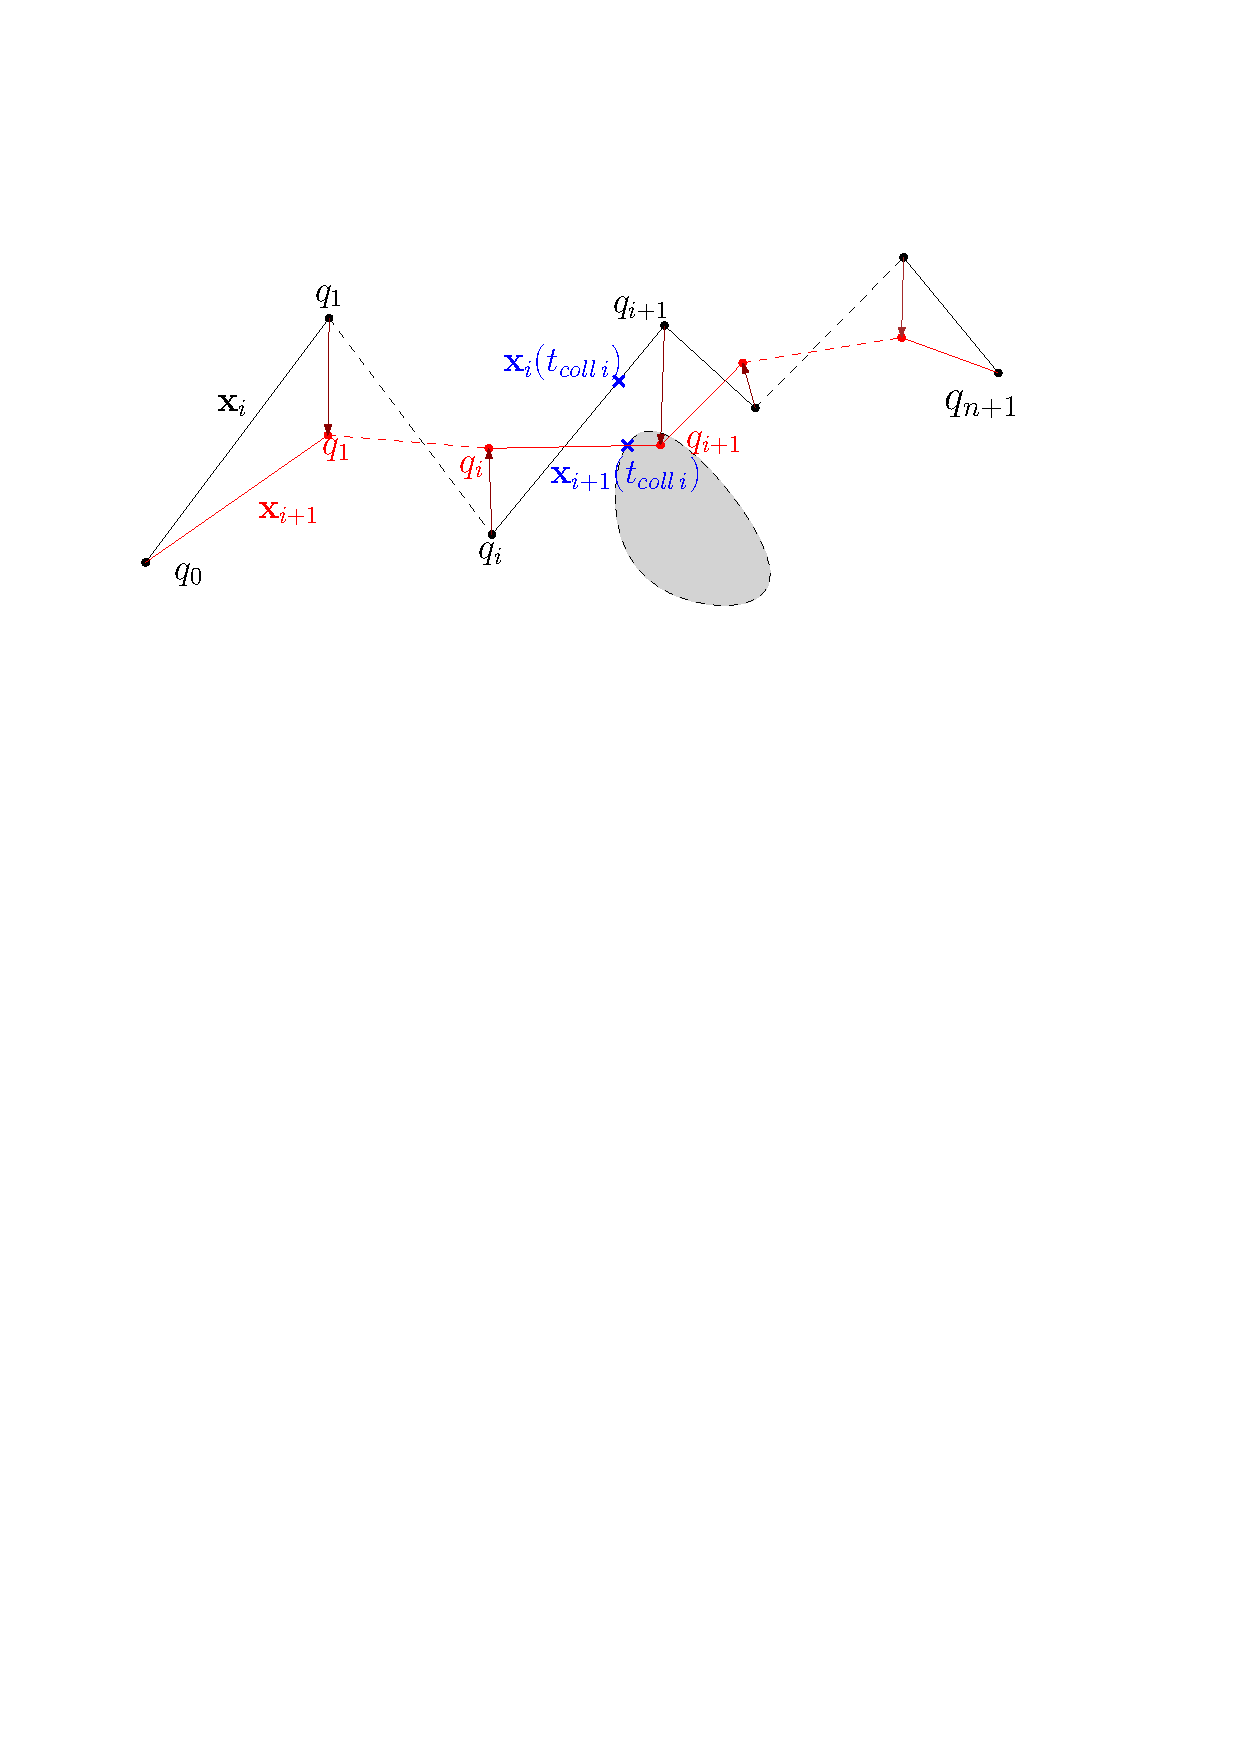
\includegraphics[width=9cm]{optim_grad.pdf}
	\caption{Illustration of one iteration of our optimization. $\xx_{i+1}$ 
	appears 
	to be in collision with the obstacle, the first colliding configuration 
	$\xx_{i+1}(\tcolli)$ is returned by the continuous collision checker. The 
	corresponding constraint will be computed in the backtracked configuration 
	$\xx_{i}(\tcolli)$.}
	\label{optim_grad}
\end{figure}

Let us assume that at iteration $i$, $k$ constraints have been inserted before the current iteration. 
These constraints are stored as lines of a Jacobian matrix as follows:
$$
\Jf_{i} = \left(\begin{array}{c}L_1 \\ \vdots \\ L_k\end{array}\right)
$$
where the step $\p_i$ is constrained to be in the kernel of $\Jf_{i}$ as follows:
$$
\Jf_{i} \p_i = 0
$$

\subsubsection{New constraint}

Each path $\xx_i$ is a mapping from 
interval $[0,1]$ into $\CS$: $\xx_i(0) = q_0$, $\xx_i(1) = q_{wp+1}$ for all $i$. As illustrated in (Figure~\ref{optim_grad}), let 
us denote by $\tcolli$ the abscissa of the first collision detected on path 
$\xx_{i+1}$, which previous iteration $\xx_i$ was collision-free. Thus in 
configuration $\xx_{i+1}(\tcolli)$ a collision has been 
detected. Two cases are possible:
\begin{enumerate}
\item the collision occurred between two bodies of the robot: $\body_1$ and $
\body_2$, or
\item the collision occurred between a body of the robot $\body_1$ and the 
environment.
\end{enumerate}
In the rest of this section, the first case will only be considered. Reasoning 
about the second case is similar, except that the 
constraint is on the position of $\body_1$ with respect to the environment.

\begin{figure}
	\centering
	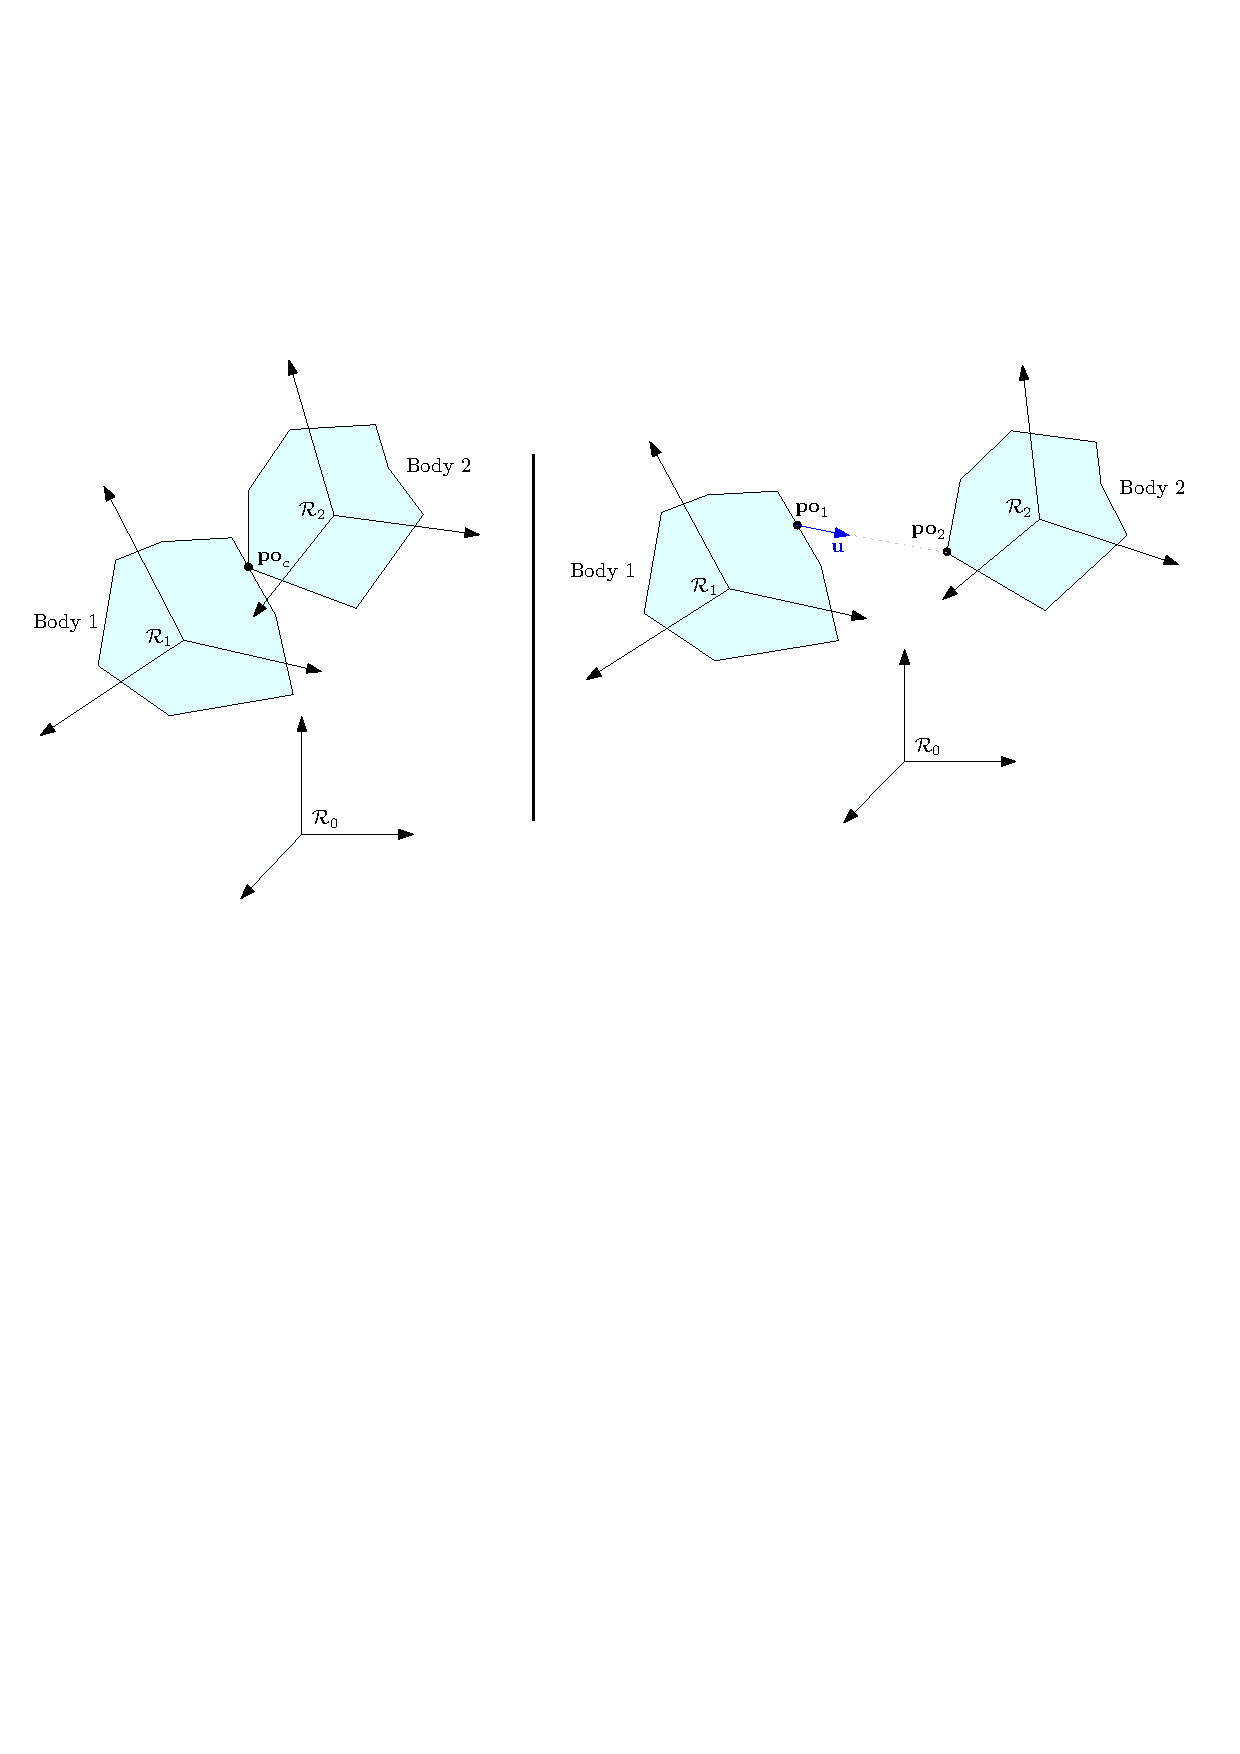
\includegraphics[width=15.8cm]{contact-points.pdf}
	\caption{Bodies representation in collision-configuration (left) and 
	backtracked free-configuration (right). A contact point (i.e. any point in 
	the intersection of the bodies) $\po_c$ can be returned by the Flexible 
	Collision Library~\cite{fcl}, used to detect collisions. The red $(\perp)$ 
	hyperplan is orthogonal to ($\po_2$,$\mathbf{u}$) and represents the motion 
	direction which is allowed by the constraint.}
	\label{contact-points}
\end{figure}

The principle of the method is to compute a constraint on the backtracked 
free-configuration $\xx_{i}(\tcolli)$ to avoid the encountered collision $\xx_{i+1}
(\tcolli)$. To handle this, we introduce a one-dimensional constraint based on the 
orthogonal direction of the encountered collision.

In the collision-configuration $\xx_{i+1}(\tcolli)$, let $\po_c\in \real^3$ be a 
contact point expressed in the global frame 
(Figure~\ref{contact-points} left). We define $\po_1$ and $\po_2$ as the coordinates of $\po_c$ in the  respective local frames of $\body_1$ and $\body_2$ (Figure~\ref{contact-points} right).

Let $M_1 \in SE(3)$ (resp. $M_2 \in SE(3)$) denote the homogeneous transformation 
between frames of $\body_1$ (resp. $\body_2$) and the global frame in configuration 
$\xx_i(\tcolli)$. Let $\mathbf{u}$ be the unit vector 
linking the contact points $\po_1$ and 
$\po_2$ in configuration $\xx_{i}(t_{coll\ i})$, $\xx_{i}$ being the latest collision-free path:
$$
\mathbf{u} = \frac{M_{1}^{-1} (\xx_i) M_2 (\xx_i) \po_2 - \po_1}{\|M_{1}^{-1} 
(\xx_i) M_2 (\xx_i) \po_2 - \po_1\|}
$$

Notice that $\mathbf{u}$ is well defined since configuration 
$\xx_{i}(t_{coll\ i})$ is collision-free.
Let $g$ be the function defined from $\CS$ to $\real$ by:
$$
g (\conf) = \left(M_{1}^{-1} (\conf) M_2 (\conf) \po_2 - \po_1 | \mathbf{u}\right)
$$
The function $g$
represents the projection of $\overrightarrow{\po_1\po_2}$ on $\mathbf{u}$ which is calculated 
from the last collision-free path at abscissa $\tcolli$.

Let $f$ be the function defined from $\CS^{wp}$ to $\real$ by:
$$
f (\xx) = g(\xx (\tcolli))
$$
The constraint is defined for any path $\xx$ by:
\begin {equation}\label{eq:new-constraint}
f(\xx) - f(\xx_{i}) = 0.
\end {equation}
This constraint forces the configuration $\xx (\tcolli)$ to keep the same distance 
between points $\po_1$ and $\po_2$ that $\xx_i (\tcolli)$. As this constraint is 
non-linear, we linearize it around $\xx_{i}$. This step is described in a further 
section. Then, a line is added in the constraint Jacobian matrix (function 
\texttt{addCollisionConstraint}), and the constraint 
Jacobian becomes:
\begin {align*}
\Jf_{i+1} &= \left(\begin{array}{c}L_1 \\ \vdots \\ L_{k+1}\end{array}\right)\ \mbox {with}\\
L_{k+1} &= \frac{\partial f}{\partial \xx}(\xx_i)
\end{align*}

\vspace{0.4cm}

Finally, we refer to~\cite{nocedal2006numerical} for solving constrained quadratic 
programs (QP) (function \texttt{computeIterate} in 
(Algorithm~\ref{algo:gradient})).

%The solution step is given by:
%$$
%\mathbf{\pii}^{*} = -V_0(V_0^TH V_0)^{-1}\,V_0^T\nabla c(\xx_i)
%$$
%where $V_0$ is the base of the nullspace of the stack of $J_F$ jacobians.

\vspace{0.2cm}

\subsubsection{Linearized constraint computation} \label{sec:lin_constr_compt}

Let $\conf_{k\,i}$ denote the waypoint $k$ along path $\xx_i$.
The constraint on the position at $t_{coll\,i}$ is a function that depends only
on two waypoints $\conf_{k\,i}$, $\conf_{k+1\,i}$, with $0\leq k\leq wp$.
There exists $\beta\in[0,1]$ such that for any $j$:
$$
\xx_j (\tcolli) = \conf_{k\,j} + \beta (\conf_{k+1\,j} - \conf_{k\,j})
$$
The path Jacobian $\frac{\partial f}{\partial \xx}(\xx_i)$ is thus built by matrix 
blocks using the previous constraint Jacobian $\frac{\partial f}{\partial \conf}$ 
and $\beta$, corresponding to \texttt{computeCollisionConstraint} in 
(Algorithm~\ref{algo:gradient}).


\subsection{Convergence Analysis}
For iterative algorithms, the risk of falling in an infinite loop 
that keeps adding a redundant constraint exists.
In this section, we give some assumptions under which our 
algorithm will converge, given the constraint definition and the 
function \texttt{solveRedundantConstraint}.
From the definition of $\Jf_{i}$, it is straightforward that:
\begin{equation}\label{eq:decreasing-kernel}
\kernel \Jf_{i+1} \subset \kernel \Jf_{i}
\end{equation}
Let us assume that:
\begin{equation}\label{eq:assumption-1}
L_{k+1}\p_i \not= 0.
\end{equation}
We will elaborate later on this assumption. This means that $\p_{i}\notin\kernel J_{i+1}$, and as $\p_{i}\in\kernel J_{i}$, then:
$$
\kernel J_i \not= \kernel J_{i+1}
$$
From~(\ref{eq:decreasing-kernel}), we deduce that:
$$
\dim (\kernel J_{i+1}) < \dim (\kernel J_i)
$$
This result proves that under assumption~(\ref{eq:assumption-1}), each added constraint 
is linearly independent from the 
previous ones, and thus our algorithm terminates in a finite number of iterations.

\vspace{0.2cm}

\subsubsection{Note about assumption~(\ref{eq:assumption-1})}%
\noindent
Let us consider the following trajectory:
\begin{equation}\label{eq:trajectory}
\conf (t) = (\xx_{i} + t\, \alpha_i \p_{i}) (t_{coll\ i}), \ t \in [0,1]
\end{equation}
where the motion is defined by taking a constant abscissa $\tcolli$ and by moving from the 
path $\xx_i$ along the step $\p_i$. Note that configuration $\xx_{i+1}(t_{coll\ i})$ is reached when $t=1$.

Thus the velocity of point $\po_2$ in the reference frame of $\body_1$ projected onto $\mathbf{u}$ along the motion of the robot is given by:
$$
 \dot{\conf}(t) = \alpha_i \frac{\partial f}{\partial \xx}(\xx_i + t\alpha_i\xx_{i+1})\p_i
$$
Therefore the following expressions
% \frac{\partial \conf}{\partial t}(0) = \alpha_i \frac{\partial f}{\partial \xx}(\xx_{i})\p_i \ \text{and} \ \frac{\partial \conf}{\partial t}(1) = \alpha_i \frac{\partial f}{\partial \xx}(\xx_{i+1})\p_i
$$
\dot{\conf}(0) = \alpha_i \frac{\partial f}{\partial \xx}(\xx_{i})\p_i \ \ \text{and} \ \ \dot{\conf}(1) = \alpha_i \frac{\partial f}{\partial \xx}(\xx_{i+1})\p_i
$$
correspond to $\dot{\po_2}(\xx).\mathbf{u}$, respectively in configurations $\xx_{i}(t_{coll\ i})$ and $\xx_{i+1}(t_{coll\ i})$. The term $\dot{\conf}(1)$ being equal to zero requires either:
\begin {enumerate}
\item that $\po_1$ and $\po_2$ come to contact at zero velocity, or
\item the velocity of $\po_2$ in the reference frame of $\body_1$ is orthogonal to 
$\mathbf{u}$ at contact ($t=1$).
\end {enumerate}
The first case is very unlikely and almost never encountered in real applications, 
except if the user builds such a case on purpose.
The second case may appear and can be noted by a rank loss of $\Jf_{i+1}$.
Then we do not directly insert the new constraint. Instead, we process intermediate 
iterations until the redundancy vanishes, as explained in function 
\texttt{findNewConstraint} and illustrated in (Figure~\ref{fig:convergence-diagram}).

\begin{algorithm}[t]
\begin{algorithmic}%[1] % line numerotation
\INPUT{$\xx_{Free}$ latest collision-free path, $\xx_{Coll}$ current path with collisions, $\p$ current iteration step}
\Require constraint $\frac{\partial f}{\partial \xx} (\xx_{Free})$ built from $\xx_{Coll}$ would produce a rank loss in constraint Jacobian $\Jf$
\State $solved \gets false$
\While{($\textbf{not}(solved)$)}
	%\State $\p = \texttt{computeIterate}()$
	%\State $minReached = (||\p||<10^{-3} \textbf{ or } \alpha=1)$
	\State $\xx \gets \xx_{Free} + 0.5\alpha\,\p$
	\If{(\texttt{validatePath}($\xx$))}
		\State $\xx_{Free} \gets \xx$
	\Else
		\State $\xx_{Coll} \gets \xx$
	\EndIf
	\State $\frac{\partial f}{\partial \xx} (\xx_{Free}) \gets$\texttt{computeCollisionConstraint}($\xx_{Coll}$, $\xx_{Free}$)
	\State $solved \gets$ \texttt{isFullRank}($\Jf$ , $\frac{\partial f}{\partial \xx} (\xx_{Free})$)
\EndWhile
\end{algorithmic}
\caption{Description of \texttt{findNewConstraint}() which returns a linearly 
independent constraint w.r.t. previous constraints stacked in $\Jf$.} 
\label{algo:solveRedundant}
\end{algorithm}

After producing an intermediate iteration $\xx_{i+2}$ where $\alpha_i$ was 
halved, the obtained path is tested for collisions. If it is collision-free, the 
constraint is now linearized around it. Otherwise, new contact points are taken 
on it, and the constraint is linearized around the latest free path.

\begin{figure}
	\centering
	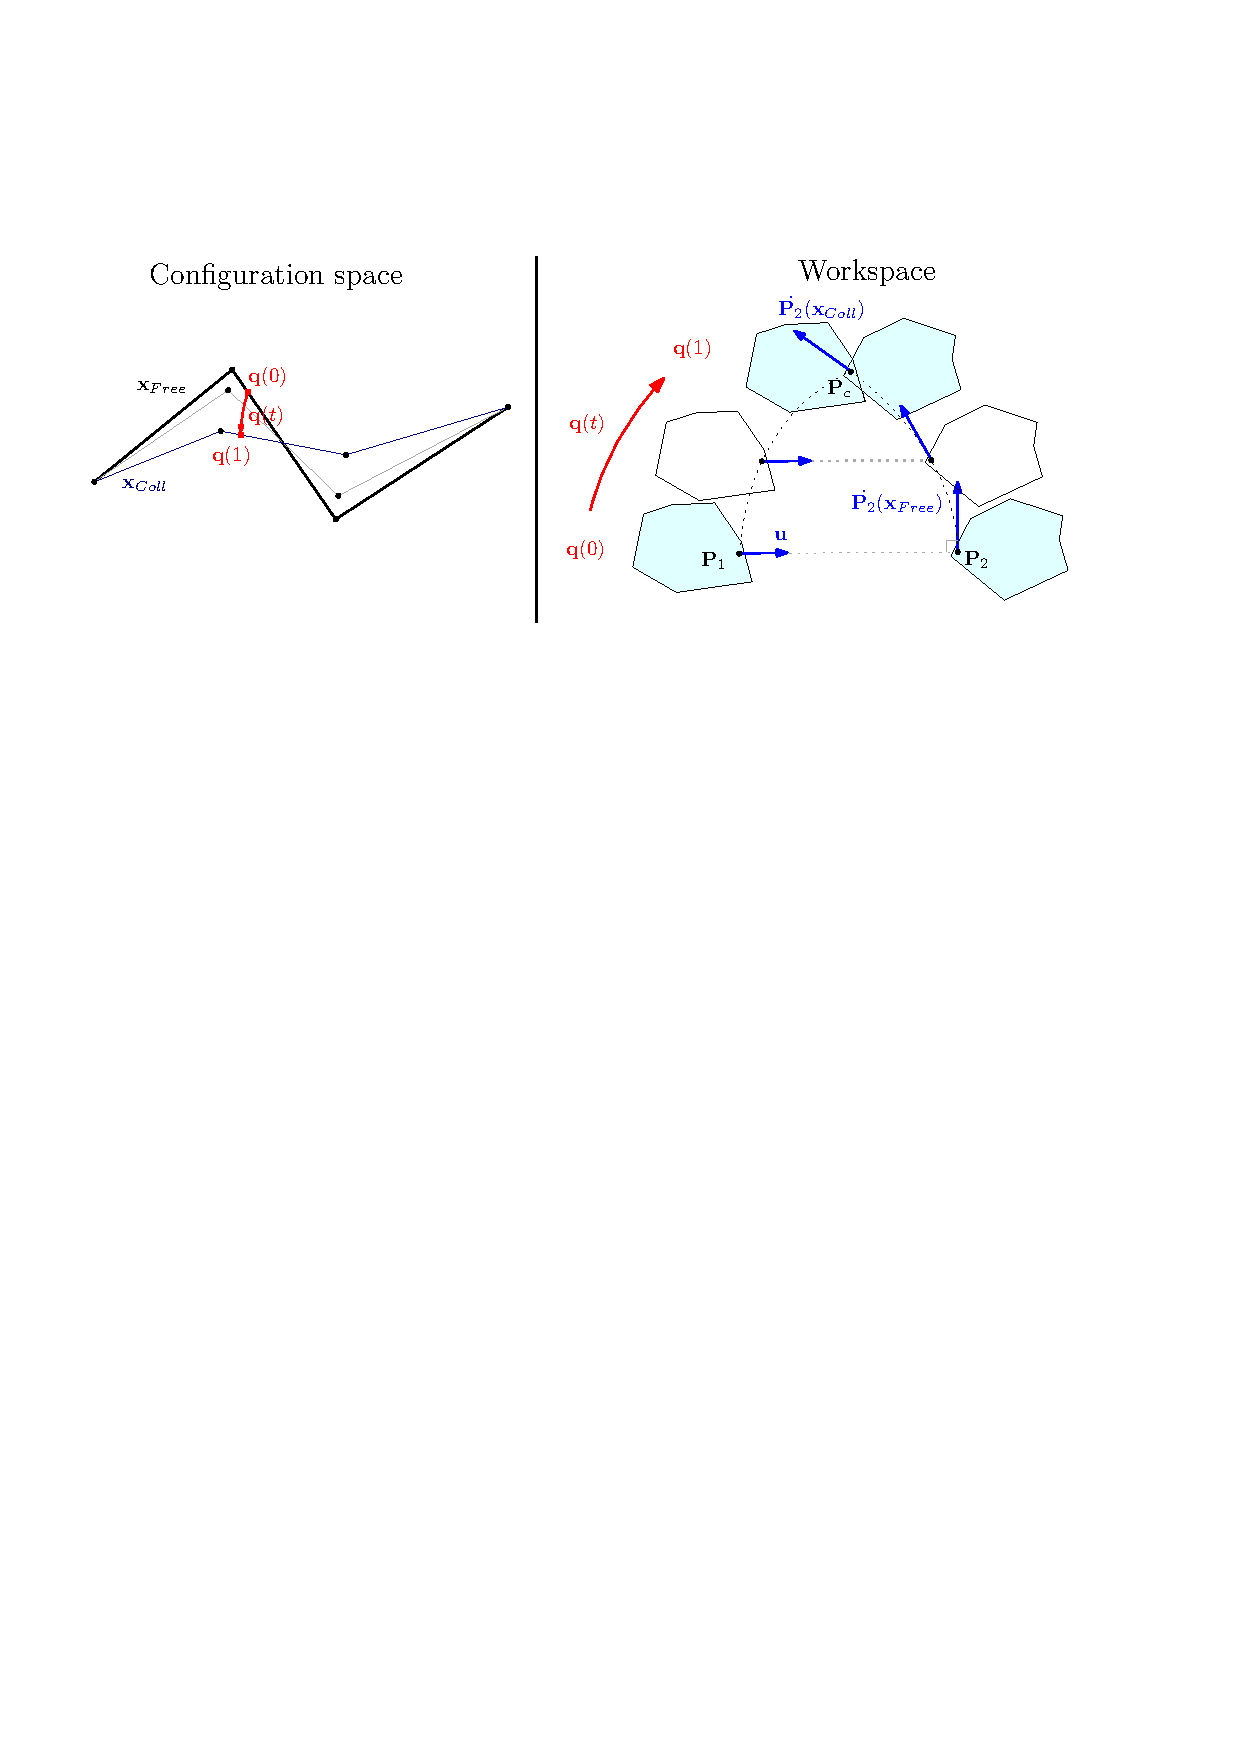
\includegraphics[width=15.8cm]{convergence-diagram.pdf}
	\caption{Representation of the trajectory $\conf (t)$ from 
	Equation~(\ref{eq:trajectory}) in the 
	configuration space (left). For the same trajectory in the workspace, the 
	colliding bodies are illustrated. Note that a case with 
	$\dot{\po_2}(\xx_{Free}).\mathbf{u}=0$ is considered. Therefore, 
	(Algorithm~\ref{algo:solveRedundant}) will produce one intermediate step
	$\xx$ (gray path and clear bodies). $\xx$ is collision-free and 
	$\dot{\po_2}(\xx).\mathbf{u}\neq 0$ so the redundancy is solved and the
	constraint will be linearized around $\xx$.}
	\label{fig:convergence-diagram}
\end{figure}

Doing so, either the new constraint makes the dimension of the kernel decrease, or 
makes the configuration in collision ($\xx_{i+1}$ or $\xx_{i+2}$ depending on the 
case above) and the latest collision-free path ($\xx_{i}$ or $\xx_{i+2}$) become 
closer and closer. And the continuity of $f$ implies that $\dot{\conf}(0)$ and 
$\dot{\conf}(1)$
converge toward the norm of the velocity of point $\po_2$ in the reference frame of 
$\body_1$ along trajectory~(\ref{eq:trajectory}) when $\po_2$ and $\po_1$ come to 
contact. We already handled this situation previously, admitting that the velocity norm 
would not vanish at $t=1$. Therefore, assumption~(\ref{eq:assumption-1}) is verified.
%$$
%\frac{\partial f}{\partial \xx}(\xx_i)\p_i \ \ \ \mbox{and}\ \ \ \frac{\partial f}{\partial \xx}(\xx_{i+1})\p_i
%$$


\subsection{Algorithm}

In this section, the GB path-optimizer (Algorithm~\ref{algo:gradient}) is described
according to the previous steps definitions. One difficulty here is to handle 
the scalar parameter $\alpha$ determining how much of the computed step $\p$ will 
be traveled along. We choose $\alpha_{init} = 0.2$ or 0.1 to process small steps.

\begin{algorithm}
\begin{algorithmic}%[1] % line numerotation
\INPUT{Path to optimize $\xx_0$}
\OUTPUT{Optimized collision-free path $\xx_0$}
\State $\alpha \gets \alpha_{init}$
\State $minReached \gets false$
\While{($\textbf{not}(noCollision \textbf{ and } minReached)$)}
	\State $\p = \texttt{computeIterate}()$
	\State $minReached = (||\p||<10^{-3} \textbf{ or } \alpha=1)$
	\State $\xx_1 \gets \xx_0 + \alpha\,\p$
	\If{(\textbf{not}(\texttt{validatePath($\xx_1$)}))}
		\State $noCollision \gets false$
		\If{$(\alpha \neq 1)$}
			\State \texttt{computeCollisionConstraint}($\xx_1$, $\xx_0$)
			\State \texttt{findNewConstraint}()
			\State \texttt{addCollisionConstraint}()
			\State $\alpha \gets 1$
		\Else
			\State $\alpha \gets \alpha_{init}$
		\EndIf
	\Else
		\State $\xx_0 \gets \xx_1$
		\State $noCollision \gets true$
	\EndIf
\EndWhile
\end{algorithmic}
\caption{Gradient-based (GB) algorithm for path-optimization.} \label{algo:gradient}
\end{algorithm}

Each time a collision-constraint is added, 
the solution of the current QP is tested (i.e. $\alpha = 1$). If this path is collision-free, the algorithm returns it as the solution. Otherwise, 
smaller steps are iteratively applied and tested toward the minimum, and constraints are added each time a collision is found with a small step (i.e. $\alpha \neq 1$).
Note that even if the constraints are linearized, the algorithm converges.


\section{RESULTS}

This part gathers optimization results performed on the planning software 
Humanoid Path Planner~\cite{hpp}. Initial paths are obtained with two 
kinds of probabilistic planners: Visibility-PRM~\cite{visibility-prm} and 
RRT-connect~\cite{rrt-connect}. Unless another value is given, $\alpha_{init}$ 
is set to 0.2.

\subsection{From 2D basic examples...}

\begin{figure}
	\centering
	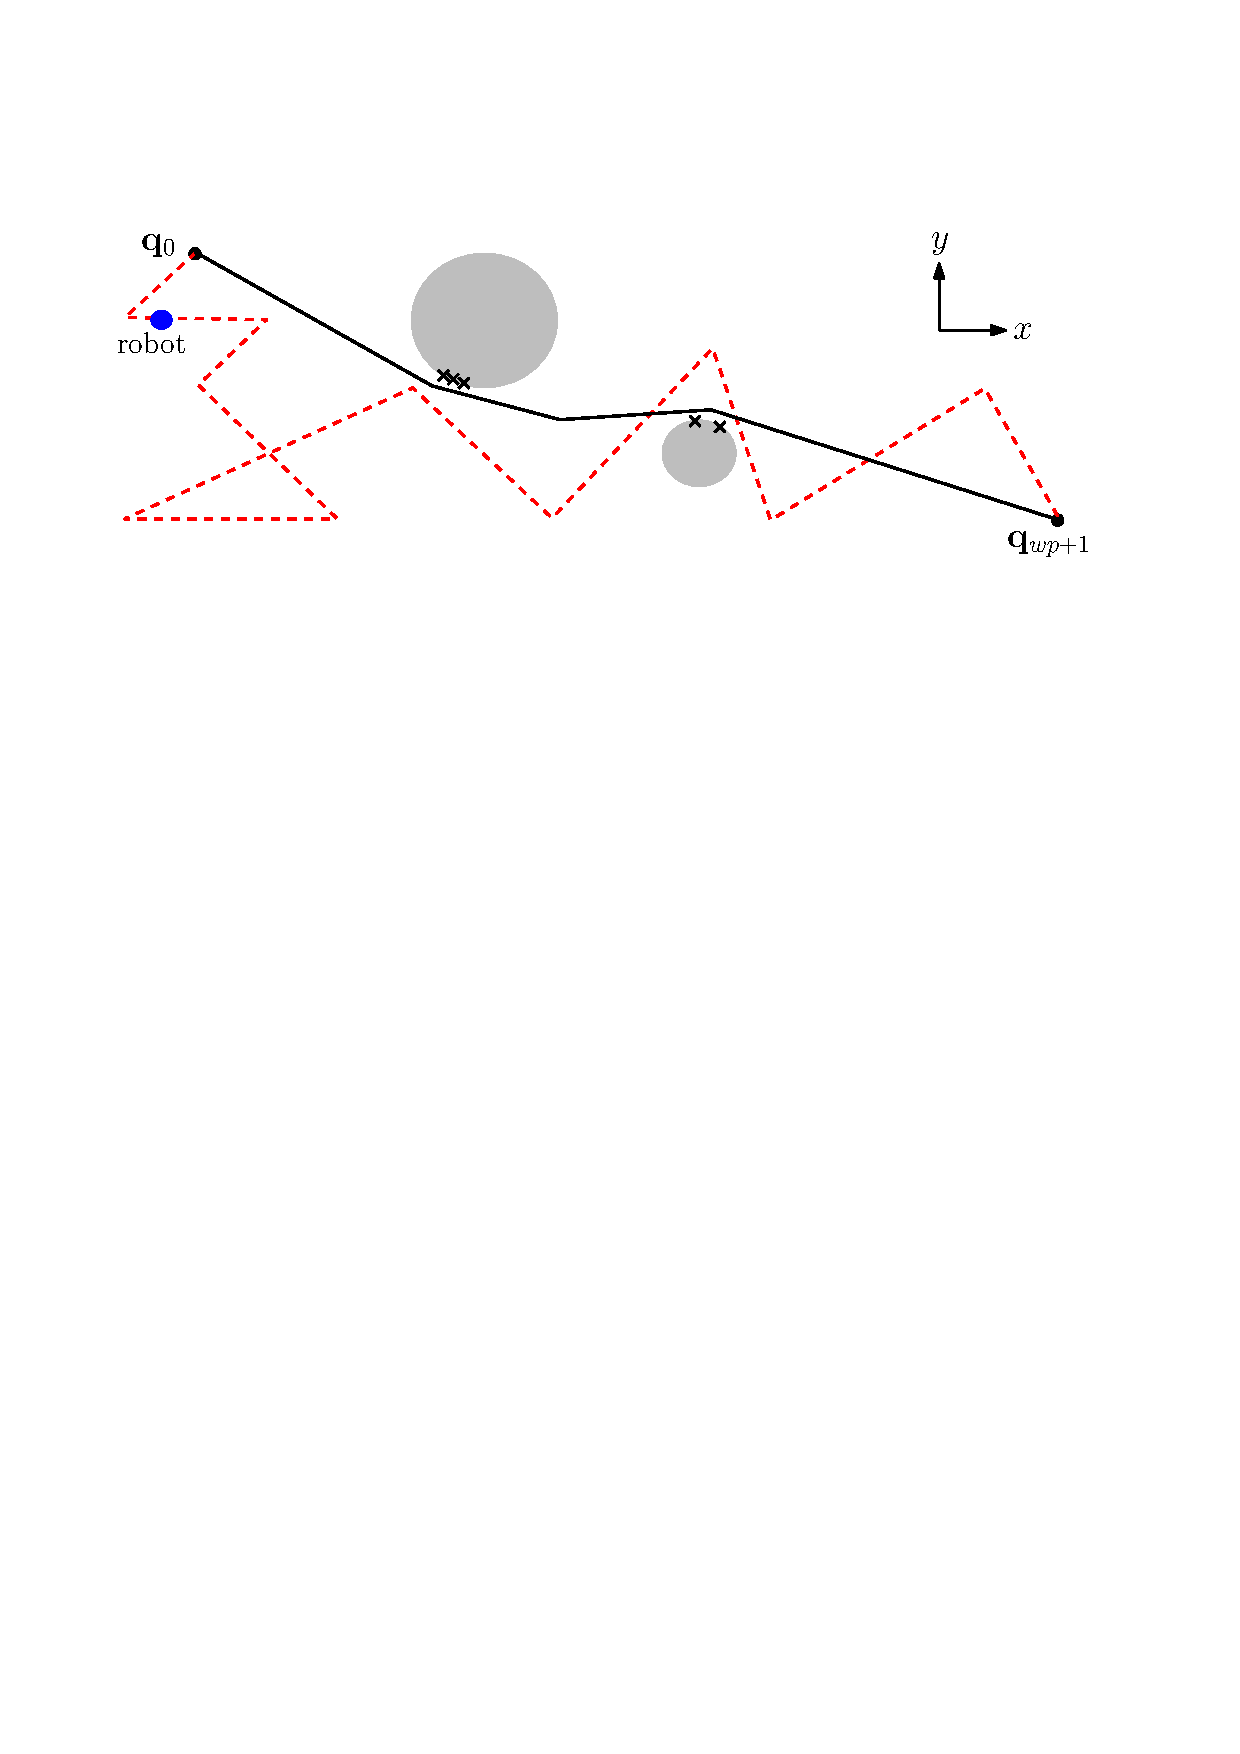
\includegraphics[width=7.8cm]{contact_points6.pdf}
	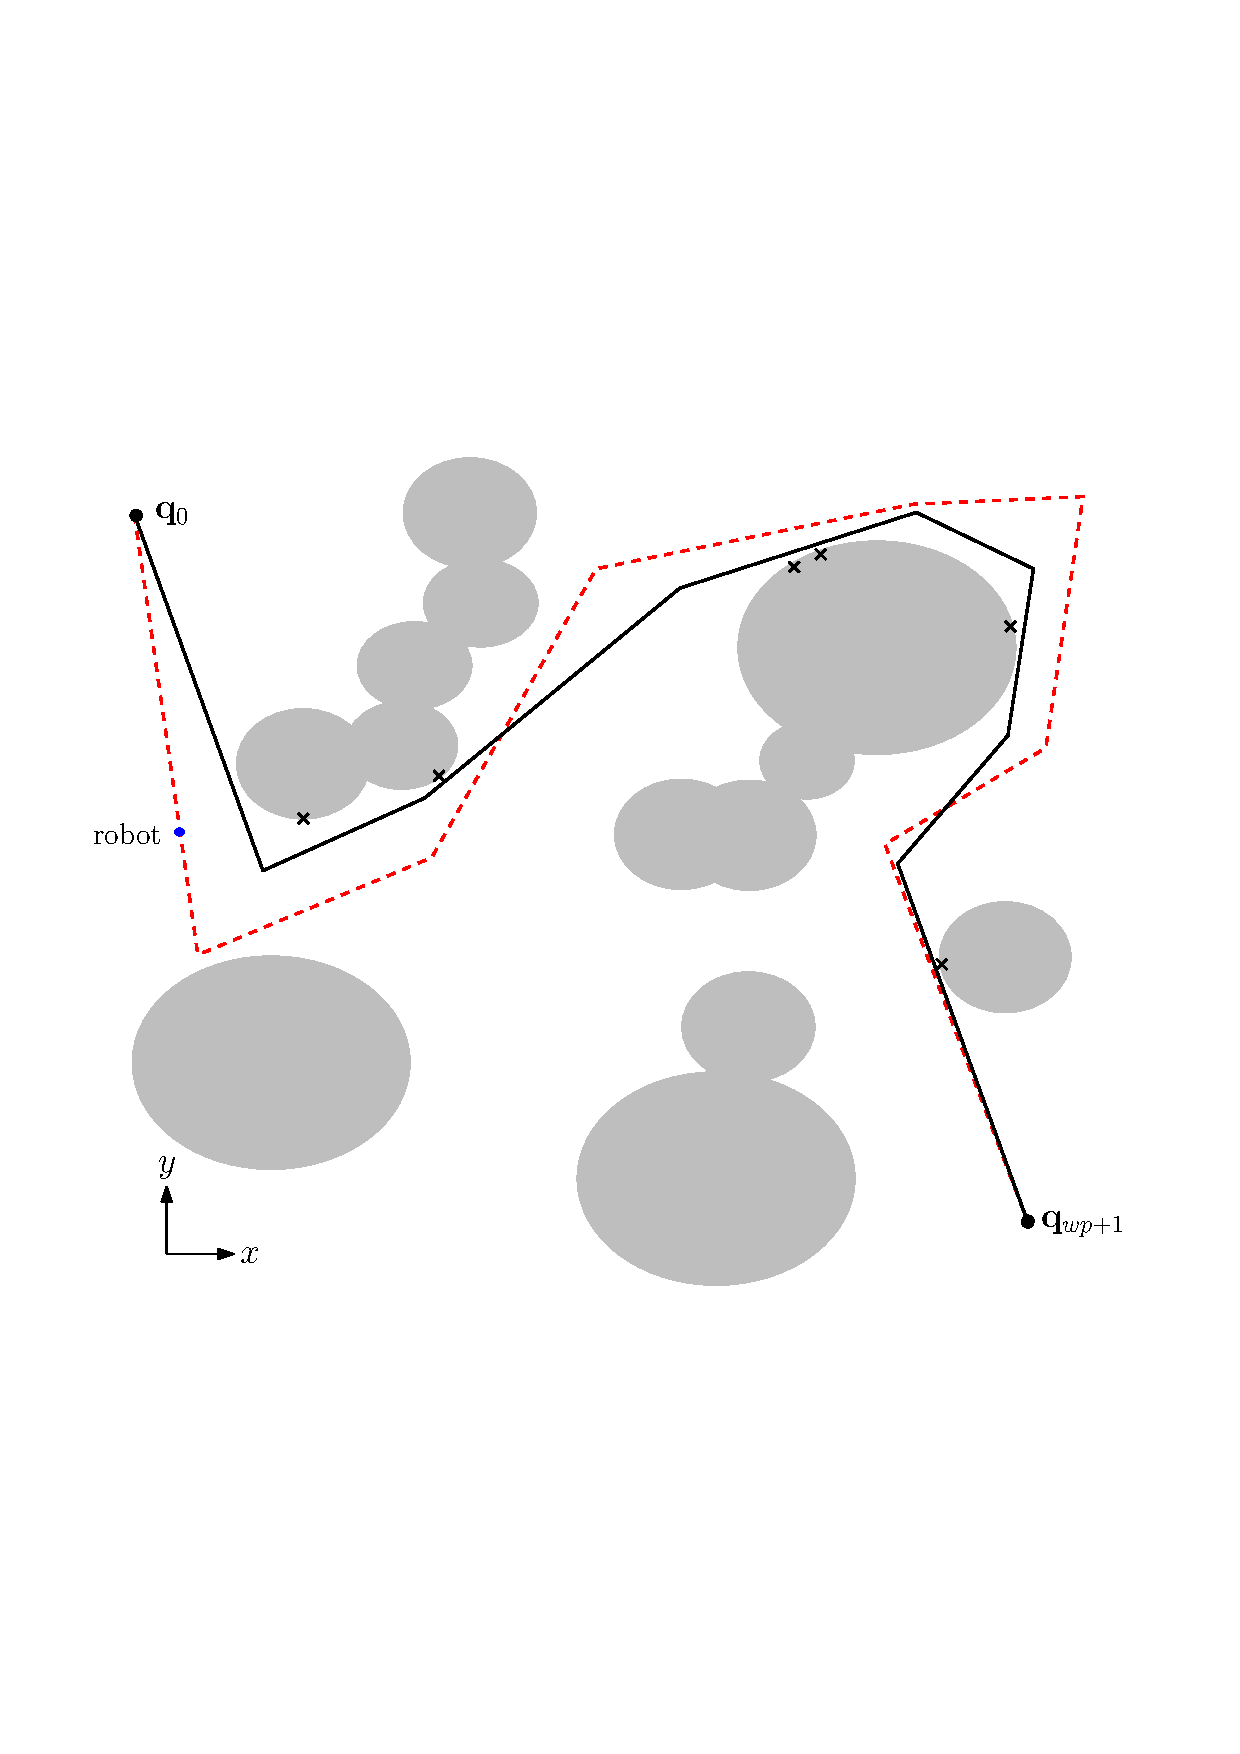
\includegraphics[width=8cm]{contact_points2potential.pdf}
	\caption{Path-optimization results on 2D robots, moving around 
	gray obstacles. Initial paths are dashed and crosses represent contact points 
	$\po_c$ related to collision-constraints. Note that, on the left, the detour 
	completely disappears.}
	\label{2D_long}
\end{figure}

(Figure~\ref{2D_long}) shows the result of our optimizer on 2D cases. Contact points which have 
led to constraints are represented. They permit to understand how the path is kept out of the obstacles. 
Unfortunately, it is not possible in the GB method to choose at which distance of the obstacle 
the constraint must be created, as at some parts the robot is very close to obstacles.

Besides, these examples give a better understanding of how the tuning of 
$\alpha_{init}$ 
has to balance lot of iterations and relevant collision-constraint addition. For 
example, if we alter a lot the initial path with a large gradient step and 
compute the corresponding collisions, constraints will be chosen on a 
path closer-to-optimality but which is not relevant
w.r.t. the obstacles we want to avoid.

(Figure~\ref{local_box_optim}) illustrates a \textit{very long} path example that RS 
or PRS will not manage to 
optimize in an affordable time, because of probabilistically failing to sample 
configurations in the box. The GB method succeeds to optimize the 
path contained in the box, with the following cost coefficients:
$$
\lambda_{i-1} = \frac{1}{\sqrt{(\conf_{i\,0}-\conf_{i-1\,0})^T \weight^2 
(\conf_{i\,0}-\conf_{i-1\,0})}}, \text{where} \  1\leq i\leq wp+1 
$$
aiming at keeping the same ratio between path segment lengths at 
minimum as at 
initial path, represented by the waypoints ($\conf_{i\,0})_{1\leq i\leq wp+1}$.
Without these coefficients, the path that minimizes the cost corresponds to a 
straight line with the waypoints equidistantly allocated, which is not adapted for 
(Figure~\ref{local_box_optim}) type of problems with a local passage very
constrained by obstacles. Note that this cost is also working with all other 
examples presented in this paper, and provides better quality results than the original cost.


\begin{figure}
	\centering
	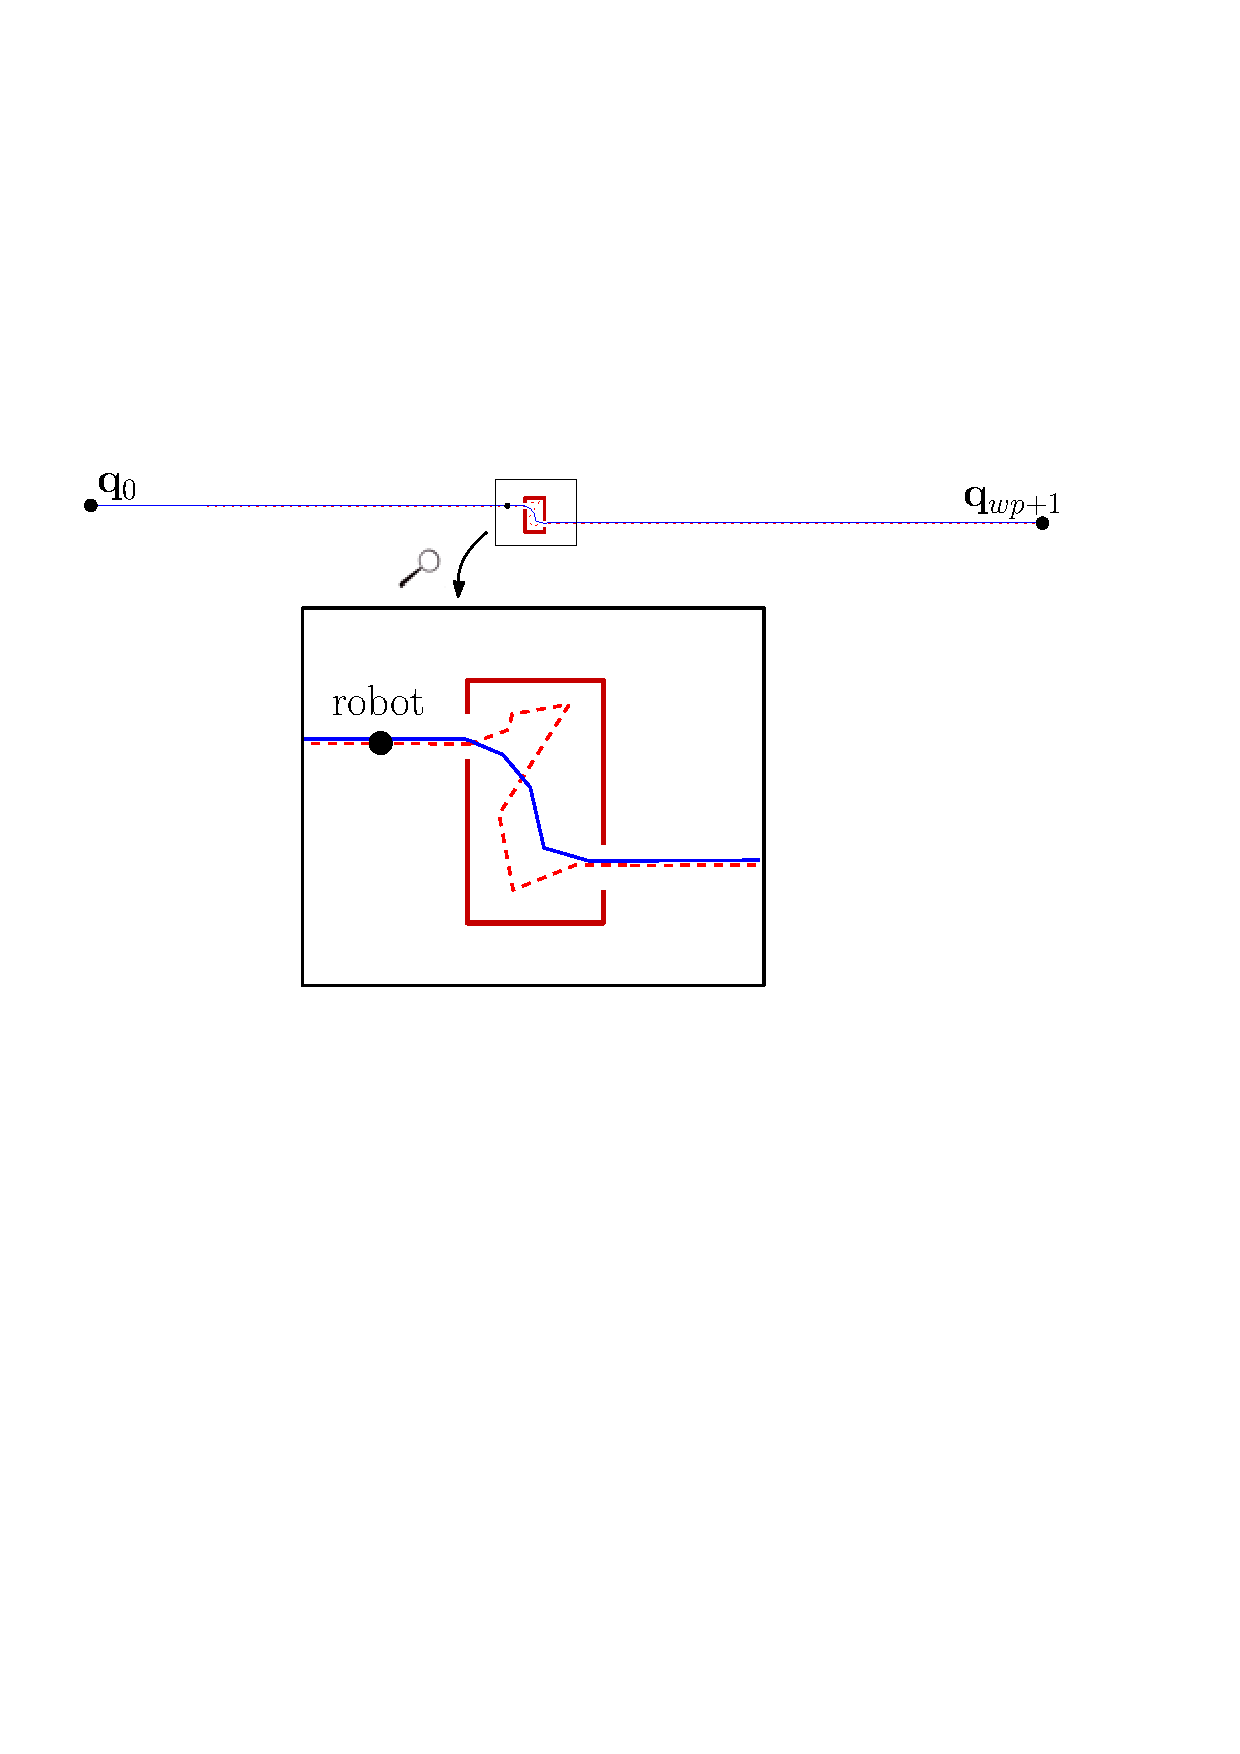
\includegraphics[width=10cm]{local_box_optim.pdf}
	\caption{Case of a long initial path (above) containing a small part 
	that can 
	be optimized (below). Random shortcut is unlikely to optimize the initial 
	dashed part containing detours in the box, whereas our method 
	succeeds (in blue). This type of issue is common in navigation problems, in 
	environments with long corridors.}
	\label{local_box_optim}
\end{figure}



\subsection{To 3D complex problems}

We also experiment our algorithm on more complex robots and environments.

\begin{algorithm}
\begin{algorithmic}%[1] % line numerotation
\INPUT{Path to optimize $\xx$}
\OUTPUT{Optimized collision-free path $\xx$}
   \State nbFailures $\gets 0$
   \While {$nbFailures < maxNbFailures$}
        \State $failure \gets true$
        \State $T \gets \mbox{upper bound of }\xx\mbox{ definition interval}$
        \State $t_1 < t_2 \gets \mbox{random numbers in }[0,T]$
        \State $lp0 \gets \texttt{steeringMethod} (\xx(0), \xx(t_1))$
        \State $lp1 \gets \texttt{steeringMethod} (\xx(t_1), \xx(t_2))$
        \State $lp2 \gets \texttt{steeringMethod} (\xx(t_2), \xx(T))$
        \State $newPath \gets \mbox{empty path defined on }[0,0]$
   	\If{$lp0$ is collision-free}
          \State $newPath \gets lp0$; $failure \gets false$
        \Else
          \State $newPath \gets \xx_{|[0,t_1]}$
        \EndIf
   	\If{$lp1$ is collision-free}
          \State $newPath \gets \texttt{concatenate} (newPath, lp1)$
          \State $failure \gets false$
        \Else
          \State $newPath \gets \texttt{concatenate} (newPath, \xx_{|[t_1,t_2]})$
        \EndIf
   	\If{$lp2$ is collision-free}
          \State $newPath \gets \texttt{concatenate} (newPath, lp2)$
          \State $failure \gets false$
        \Else
          \State $newPath \gets \texttt{concatenate} (newPath, \xx_{|[t_2,T]})$
        \EndIf
        \State $\xx \gets newPath$
        \If {$failure$} $nbFailures \gets nbFailures + 1$
        \EndIf
      \EndWhile
    \Return $\xx$
\end{algorithmic}
\caption{Random shortcut as adapted from~\cite{Sekhavat-Svestka1998} 
Section~6.4.1. \texttt{steeringMethod} returns the linear interpolation between 
two configurations. $\xx_{|I}$ denotes path $\xx$ restricted to interval $I$. 
$maxNbFailures$ is a parameter that affects time of computation and quality of 
the result.}\label{algo:random-shortcut}
\end{algorithm}

\begin{figure}
	\centering
	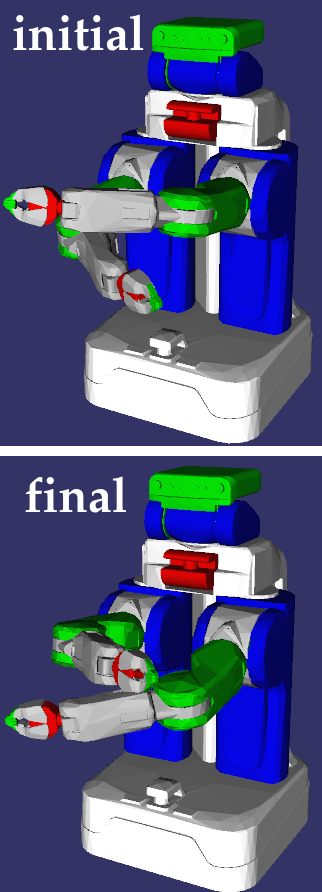
\includegraphics[height=4.9cm,width=1.8cm]{pr2_initial_final_vertical.png}
	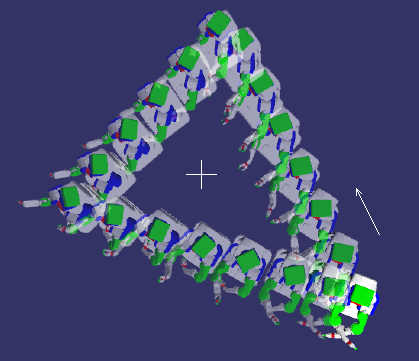
\includegraphics[width=5.7cm]{p0_pr2_alone_merged3.png}
	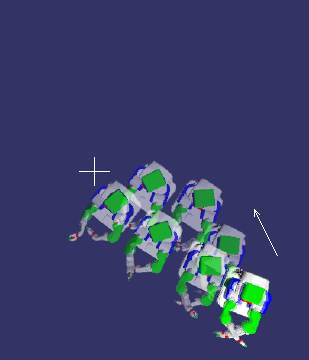
\includegraphics[height=4.9cm]{p1RS_pr2_alone_merged3.png}
	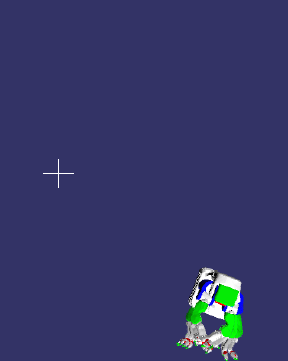
\includegraphics[height=4.9cm]{p1GB_pr2_alone_merged3.png}\\
	\caption{PR2-crossing-arms example. In this motion planning problem, PR2 robot 
	has just to 
exchange the positions of its arms. The task is simple, however, in absence of 
explicit indication, any probabilistic motion planner will compute a path that 
makes the PR2 mobile base purposelessly moving. This is the result of RRT-connect 
algorithm (left). Path optimization is expected to remove unnecessary motions. 
The popular RS algorithm fails in this case (middle). Our GB algorithm 
succeeds (right).}
	\label{pr2_final}
\end{figure}

In the included video and (Figures~\ref{pr2_final},~\ref{fiad} 
and~\ref{fig:trajectories}), we present multiple situations where the GB algorithm 
is tested and compared to RS~\cite{randomShortcutHPP}
(Algorithm~\ref{algo:random-shortcut}) and PRS~\cite{partialrandomShortcutHPP} 
adapted from~\cite{Geraerts04clearancebased}.
The termination condition of RS allows it to try 
shortening the path until five iterations of non-improvement are reached 
(corresponding to $maxNbFailures$ in (Algorithm~\ref{algo:random-shortcut})).
For our implementation of PRS, first a shortcut is tried on each DOF between 
$\conf_0$ and $\conf_{wp+1}$. 
Then, for each DOF, configurations are sampled as in 
(Algorithm~\ref{algo:random-shortcut}). The steering-method returns a path made of 
an interpolation on only 
the current DOF and based on the previous subpath for other DOF. If this path is 
collision-free, we replace it as in RS. This process is also stopped when five 
iterations of non-improvement are reached.

\vspace{0.4cm}
% freeflyer puzzle
Before entering the manipulator examples, the GB algorithm is tested and compared 
on a problem very popular in the motion planning literature: a freeflyer puzzle 
example, corresponding to (Figure~\ref{fig:trajectories:puzzle}).  The puzzle has to cross down the 
obstacle using the hole in the middle. The initial path planned with Visibility-PRM 
contains detours above and below the obstacle, as well as small superfluous
motions in the hole. 
Lengths of initial, GB optimized, and RS optimized paths are 
respectively 23.4, 8.53 and 10.2. PRS fails to decrease the path length because in 
this problem, all DOF are closely related to cross the hole. This behavior was also 
noticed and improve in the PRS implementation of~\cite{Geraerts04clearancebased}, 
acting on a group of DOF. The GB optimizer manages to modify the puzzle trajectory 
even in the hole, contrary to RS which simply copies the initial path when the 
trajectory gets near of the obstacle. $\alpha_{init}$ is reduced to 0.05 to slightly modify the very constrained trajectory at each iteration.

\vspace{0.4cm}

% double-arm:
On the double-arm problem, (Figure~\ref{fig:trajectories:double_arm}), one arm has 
to get around a cylinder obstacle while the 
other arm is relatively far from obstacles. As expected, the initial path given by 
RRT-connect activates both arms to solve the problem. Unlike RS, 
the GB optimizer manages to cancel the rotation of the free-arm while optimizing the 
first arm motion, even if the second arm is still moving because of the translation 
motion. The initial path length 5.17 is decreased to 4.55 by RS, to 4.06 by PRS and 
to 2.77 by the GB method using three collision-constraints with the cylinder obstacle.


\begin{figure}
	\centering
	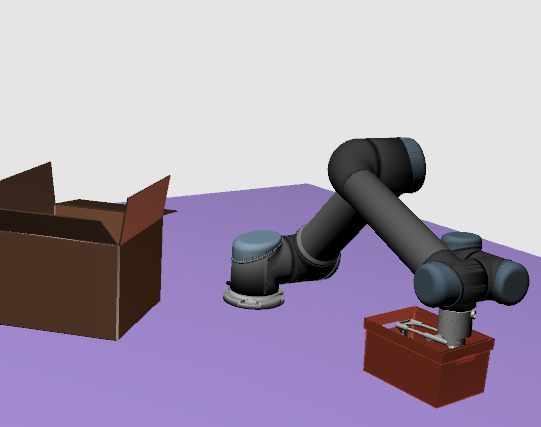
\includegraphics[width=5.8cm,height=4.7cm]{fiad_qinit.png}
	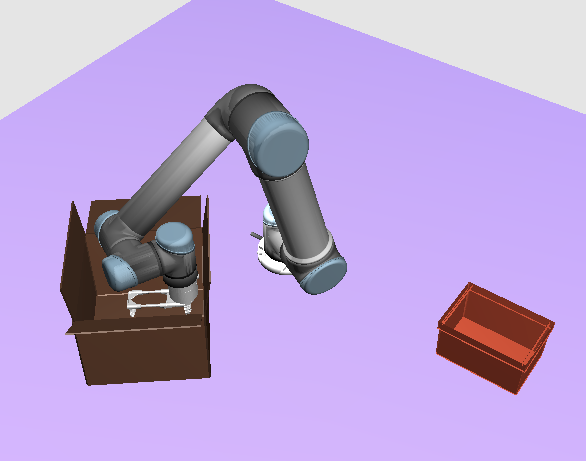
\includegraphics[width=5.8cm,height=4.7cm]{fiad_qfinal.png}\\
	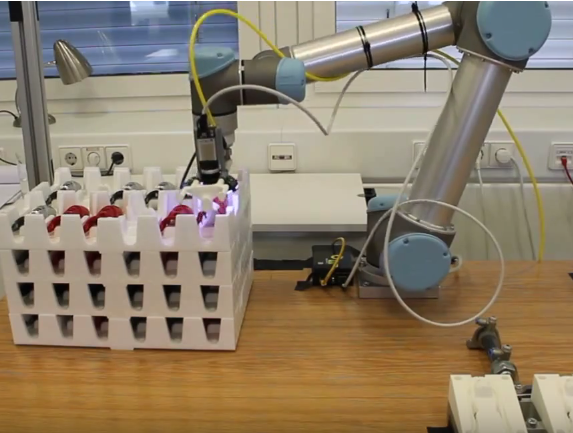
\includegraphics[width=5.8cm,height=4.7cm]{fiad_real.png}
	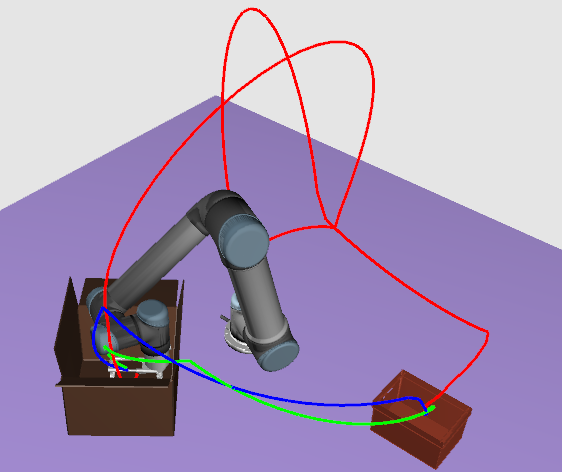
\includegraphics[width=5.8cm,height=4.7cm]{fiad-trajectorires.png}
	\caption{(Bottom left) An industrial use-case example proposed by Philips for 	
	the Factory-in-a-Day project~\cite{factory-day-video}. A similar environment 	
	has been created (top) to illustrate that our method can comply with an 
	industrial problem, where initial and final configurations of the UR5 are 
	constrained in boxes. Trajectories results 
	are presented (bottom right): initial (RRT-connect) path in red, RS 
	optimization in blue and the GB optimization in green.}
	\label{fiad}
\end{figure}

% UR5-spheres:
Some problems are 
involving a 6-axis manipulator arm, also called UR5, equipped with a bar or a 
gripper.
In a relatively free environment (Figure~\ref{fig:trajectories:ur5}), 
results from our method and RS are similar (path length are respectively 2.03 and 1.60). 
Note also that the end-effector trajectory is completely different from the initial 
one: the robot is easily passing between the spheres, keeping its end-effector 
above.

% UR5-fiad
For an UR5 working in a cluttered environment inspired by an industrial issue 
(Figure~\ref{fiad}), path optimization efficiently returns a shorter solution, close 
to the result of RS and to what can be observed in reality~\cite{factory-day-video}. 
The initial path length 6.65 is decreased to 2.08 by RS, to 
1.98 by the GB optimizer and unchanged by PRS.

% baxter:
A problem involving a Baxter-like\footnote{A torso rotation was added.} robot 
manipulating in an office environment is presentated 
(Figure~\ref{fig:trajectories:baxter}). The robot starts with its end-effectors 
above the computer and has to 
turn and reach the shelf. According to the left-hand trajectories quality (see the 
video for the full motion) and path lengths, 9.10 (initial RRT-connect), 7.52 (RS), 
8.41 (PRS) and 2.70 (GB), the GB optimizer is the most successful in this case.

\vspace{0.4cm}

On the three following high-DOF examples involving the PR2 robot, we argue that 
results are better in terms of path quality, in the fact that parasite DOF motions 
are removed.

% analysis PR2 alone:
In the example presented (Figure~\ref{pr2_final}) and in the video, the mobile 
40-DOF PR2 simply has to cross its arms from 
the left arm up position to the right arm up one, without any assumption on the DOF or group of DOF to choose to plan or optimize (i.e. no DOF is locked). 
The RRT-connect planner 
returns detours and activates non-useful DOF such as the head, the torso lift 
and the translation on the ground. Such behavior induces a high initial path length 
30.6. RS hardly optimizes the mobile base 
translation (Figure~\ref{pr2_final} middle) of the robot and other unnecessary DOF 
uses, resulting in a path length of 4.08.
Whereas the GB optimized-path mainly 
results in moving the arms as expected (Figure~\ref{pr2_final} right), just creating 
two collision-constraints between the arms. The PRS 
result, only presented in the video, cancels the mobile base motion, but not all 
unnecessary DOF. In addition, the arms motion is very wide and not as optimized as in the GB trajectory.

% analysis PR2 in kitchen:
We obtain similar results on the PR2 performing a manipulation task 
in a kitchen environment (see the video and (Figure~\ref{fig:trajectories:kitchen1}) 
to visualize the trajectory of the right gripper). The robot has to move 
its hands from the top to the bottom of a table.
Our optimizer manages to reduce the initial length 12.7 from the visibility-PRM 
planner and improves the path quality 
just adding orthogonality constraints between the table and the 
robot's arms and grippers. Thus, the robot just slightly moves 
backward and uses its arms DOF to avoid the table, instead of 
processing a large motion to get away from the table. With the GB algorithm, the path length is 
downed to 3.15, against 5.47 for RS.
Another example of PR2 working in the kitchen, going from the set to the fridge 
door, is presented (Figure~\ref{fig:trajectories:kitchen2}) with the mobile base
trajectories. Here, GB and RS results are similar in terms of length and rendering.

\vspace{0.4cm}

Optimization computation time and path length averages are presented for 30 runs of 
each example in (Table~\ref{tab:results}). In some cases $\alpha_{init}$ was 
reduced to comply with very narrow passages, or increased in the opposite case. 
On the one hand, for non-high DOF examples, it appears that computation time is higher using the GB 
optimization. The worst case comes out for the puzzle problem where the number of 
constraints of GB is significant and $\alpha_{init}$ reduced. 
In addition, collision checking is rapidly processed in such basic problem geometry. This favors RS while the GB optimization spends time on the QP resolution to avoid collisions.
On the other hand, our method almost always provides the shortest paths, whereas it 
is not even the best criterion to quantify the parasite motions disappearance.
Such results are the artefact of the termination conditions of RS and PRS, length 
reduction or affordable computation time. This is particularly visible for PRS which 
easily gives up in some problems, such as the 2D sliding-robot, the 
UR5-with-spheres or the puzzle.
Finally, the complete vanishing of the mobile base motion in the PRS and GB 
optimized paths is highlighted in the right column of (Table~\ref{tab:results}). 
Thus the problem addressed in (Figure~\ref{decoupled_DOF_optimization}) is 
solved considering this DOF.



\begin{figure}
	\centering
	\subfigure[Double-arm]{
		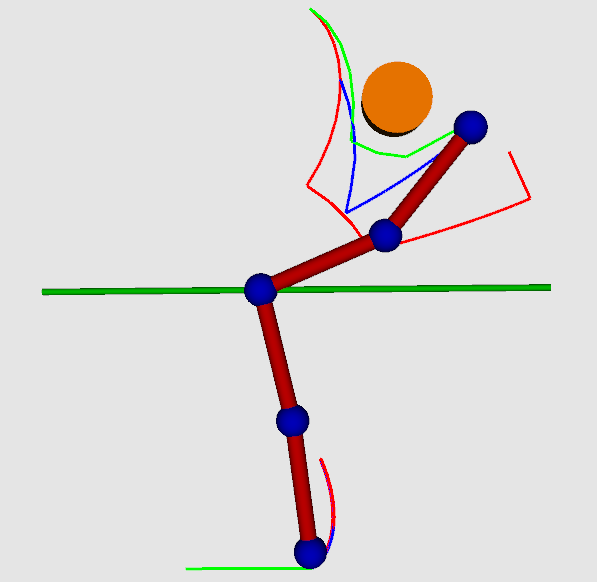
\includegraphics[width=6.5cm,height=5.5cm]{ur2_orth_constr_results.png}
		\label{fig:trajectories:double_arm}
	}
	\subfigure[Freeflyer-puzzle]{
		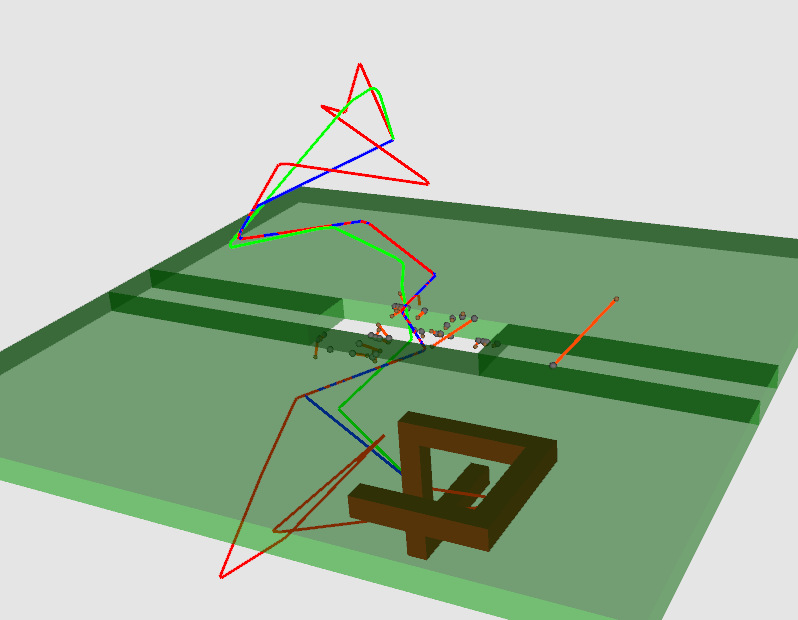
\includegraphics[width=6.5cm,height=5.5cm]{puzzle_orth_constr_results.png}
		\label{fig:trajectories:puzzle}
	}
	\subfigure[PR2-in-kitchen-1]{
		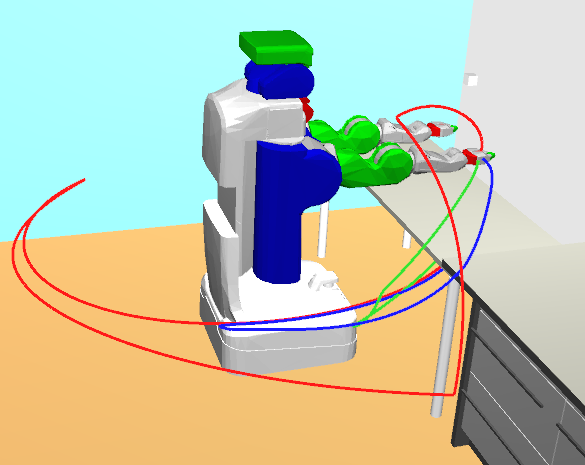
\includegraphics[width=6.5cm,height=5.5cm]{pr2-kitchen1_orth_constr_results.png}
		\label{fig:trajectories:kitchen1}
	}
	\subfigure[UR5-with-spheres]{
		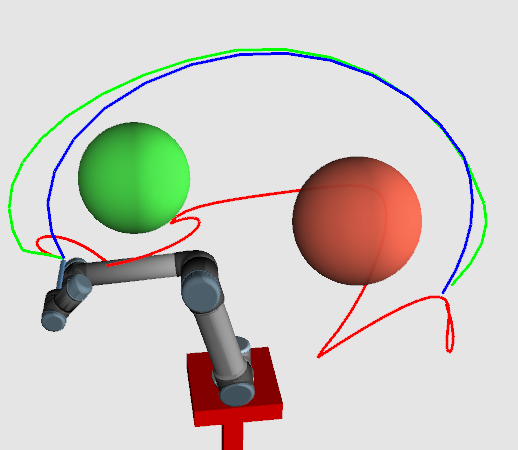
\includegraphics[width=6.5cm,height=5.5cm]{ur5-spheres_orth_constr_results.png}
		\label{fig:trajectories:ur5}
	}
	\subfigure[PR2-in-kitchen-2]{
		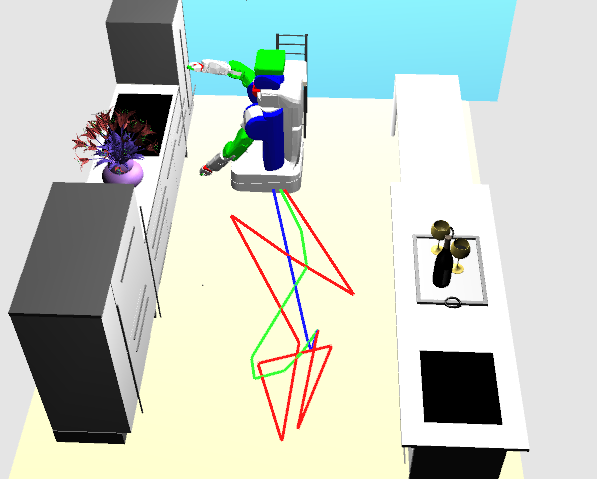
\includegraphics[width=6.5cm,height=5.5cm]{pr2_kitchen2_orth_constr_results.png}
		\label{fig:trajectories:kitchen2}
	}
	\subfigure[Baxter-in-office]{
		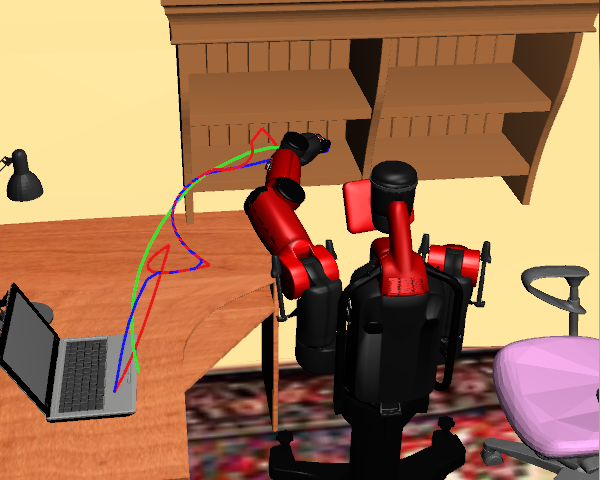
\includegraphics[width=6.5cm,height=5.5cm]{baxter_orth_constr_results.png}
		\label{fig:trajectories:baxter}
	}
  \caption{Trajectories of end-effectors, mobile bases or centers along the 
  different paths: the initial path is represented in red, the RS optimized path in 
  blue and the GB optimized path in green. The full robots 
  motions can also be visualized in the joined video. The trajectories comparison 
  highlights the optimization success of our method, which manages to deliver a 
  shorter or similar path compared to RS output}
  \label{fig:trajectories}
\end{figure}



\begin{table}
\centering
\scalebox{0.9}{
  \begin{tabular}{ccccc}
  \toprule
    \textbf{Problem} & Path obtained from & Computation time  & Path length & Base traveled distance\\
    \midrule
    \midrule
    & Initial &  & $21.9$  &\\
    \textbf{2D slidding-robot} & GB & $9.29\,\text{ms}$ & $17.0$  &\\
    \textbf{(Fig.~\ref{2D_long} right)} & PRS & $0.336\,\text{ms}$ & $21.7$  &\\
    & RS & $1.89\,\text{ms}$ & $17.7$  &\\
    \midrule
    & Initial &  & $18.8$  &\\
    \textbf{Freeflyer-} & GB ($\alpha_{init}=0.05$) & $1020\,\text{ms}$ & $9.65$  &\\
    \textbf{puzzle} & PRS & $1.13\,\text{ms}$ & $18.8$  &\\
    & RS & $4.72\,\text{ms}$ & $10.3$  &\\
    \midrule
    & Initial &  & $10.8$  &\\
    \textbf{Double-arm} & GB & $10.3\,\text{ms}$ & $4.79$  &\\
    \textbf{5-DOF} & PRS & $2.17\,\text{ms}$ & $8.08$  &\\
    & RS & $5.33\,\text{ms}$ & $6.24$  &\\
    \midrule
    & Initial (RRT) &  & $4.97$ &\\
    \textbf{UR5-} & GB ($\alpha_{init}=0.4$) & $2.12\,\text{s}$ & $2.97$ &\\
    \textbf{with-spheres} & PRS & $0.884\,\text{s}$ & $4.56$ &\\
    & RS & $2.89\,\text{s}$ & $2.99$ &\\
    \midrule
    & Initial &  & $4.83$ &\\
    \textbf{UR5-} & GB ($\alpha_{init}=0.4$) & $314\,\text{ms}$ & $2.25$ &\\
    \textbf{industrial-example} & PRS & $30.2\,\text{ms}$ & $4.53$ &\\
    & RS &  $95.6\,\text{ms}$ & $2.16$ &\\
    \midrule
    & Initial &  & $20.2$ &\\
    \textbf{Baxter-in-} & GB & $22.7\,\text{s}$ & $6.65$ &\\
    \textbf{office} & PRS & $9.49\,\text{s}$ & $18.9$ &\\
    & RS & $3.13\,\text{s}$ & $11.9$ &\\
    \midrule
    & Initial &  & $12.6$  & $9.57$\,\text{m}\\
    \textbf{PR2-crossing-} & GB & $1.28\,\text{s}$ & $2.57$  & $0\,\text{m}$\\
    \textbf{arms} & PRS & $2.63\,\text{s}$ & $ 5.31$ & $0\,\text{m}$\\
    & RS & $1.92\,\text{s}$ & $3.59$ & $2.63\,\text{m}$\\
    \midrule
    & Initial &  & $15.3$ &\\
    \textbf{PR2-in-} & GB & $19.2\,\text{s}$ & $4.53$ &\\
    \textbf{kitchen-1} & PRS & $23.5\,\text{s}$ & $12.2$ &\\
    & RS & $9.88\,\text{s}$ & $5.75$ &\\
    \bottomrule
  \end{tabular}
  }%scalebox
\caption{Average results for 30 runs of several examples presented in the paper and 
in the video. For each run, a solution path is planned by Visibility-PRM (unless 
`RRT' for RRT-connect is mentioned) as initial guess for each optimizer.
For the PR2-crossing-arms example only, the right column represents the 
distance that is traveled by the robot mobile base during the different paths.
}
\label{tab:results}
\end{table}



\section{CONCLUSIONS}
We managed to settle a path optimization for navigation and manipulation problems, and tested it with various robots and environments. Our algorithm uses standard 
numerical tools as collision checking, linearized one-dimensional constraint
and QP resolution. It correlates them in a 
simple but effective way, and the algorithm structure is organized so that the convergence is guaranteed. Furthermore, 
our method only requires collision checking, therefore geometry pre-processing or 
offline optimization are not necessary to remain time-competitive. We demonstrate 
that the optimizer may be 
time-competitive compared to random shortcut in complex models where collision tests are time-consuming. 
It also proposes better quality paths, reducing the path length and removing unnecessary DOF motions. 
Finally, our optimizer manages to reduce a local detour in a long path while random shortcut methods will mostly fail.

For future work, we have room for improvement: taking advantage of the sparsity of 
the constraint Jacobian to reduce computation time. We may also adapt the iteration 
scalar parameter from geometries considerations on the current path, e.g. a lower 
bound of the distance between nearest objects, since this bound can be returned by 
the collision checker.


\section*{Funding}
This work has been supported by the project ERC Advanced Grant 340050 Actanthrope and by the FP~7 project Factory in a Day under grant agreement n°~609206.


\bibliographystyle{tADR}
\bibliography{paper}

\end{document}
